\documentclass[journal]{IEEEtran}

% *** CITATION PACKAGES ***
%
%\usepackage{cite}
\usepackage{capt-of}%%To get the caption
\usepackage{gensymb}
\usepackage{graphicx} %package to manage images
\graphicspath{ {./images/} }
\usepackage{wrapfig}

\usepackage[style=ieee]{biblatex}
\DeclareLanguageMapping{english}{english-apa}
\addbibresource{references.bib}
\usepackage[justification=centering]{caption}

\usepackage{setspace}

\usepackage{hhline}

\usepackage{booktabs}

% *** GRAPHICS RELATED PACKAGES ***
%
\ifCLASSINFOpdf
  % \usepackage[pdftex]{graphicx}
  % declare the path(s) where your graphic files are
  % \graphicspath{{../pdf/}{../jpeg/}}
  % and their extensions so you won't have to specify these with
  % every instance of \includegraphics
  % \DeclareGraphicsExtensions{.pdf,.jpeg,.png}
\else
  % or other class option (dvipsone, dvipdf, if not using dvips). graphicx
  % will default to the driver specified in the system graphics.cfg if no
  % driver is specified.
  % \usepackage[dvips]{graphicx}
  % declare the path(s) where your graphic files are
  % \graphicspath{{../eps/}}
  % and their extensions so you won't have to specify these with
  % every instance of \includegraphics
  % \DeclareGraphicsExtensions{.eps}
\fi
% graphicx was written by David Carlisle and Sebastian Rahtz. It is
% required if you want graphics, photos, etc. graphicx.sty is already
% installed on most LaTeX systems. The latest version and documentation
% can be obtained at: 
% http://www.ctan.org/pkg/graphicx
% Another good source of documentation is "Using Imported Graphics in
% LaTeX2e" by Keith Reckdahl which can be found at:
% http://www.ctan.org/pkg/epslatex
%
% latex, and pdflatex in dvi mode, support graphics in encapsulated
% postscript (.eps) format. pdflatex in pdf mode supports graphics
% in .pdf, .jpeg, .png and .mps (metapost) formats. Users should ensure
% that all non-photo figures use a vector format (.eps, .pdf, .mps) and
% not a bitmapped formats (.jpeg, .png). The IEEE frowns on bitmapped formats
% which can result in "jaggedy"/blurry rendering of lines and letters as
% well as large increases in file sizes.
%
% You can find documentation about the pdfTeX application at:
% http://www.tug.org/applications/pdftex

\begin{document}

\begin{titlepage}
    {\centering
        \vspace*{20em}
        {
        \huge 
        \begin{spacing}{1.5}
            Lab Report \#1: Operational Amplifiers
            \\
            Advanced Circuits Lab (ENGR$-$UH 2311),\\
            Spring 2019
            \bigskip
            \Large
            \\
            Determining the Characteristics of Various\\
            Operational Amplifier Circuit Configurations
  
            \\
            \bigskip
            Deadline: April 17, 2019 
        \end{spacing}

        }
        
    }
    \vfill
    
    {
    \large
    
    \begin{spacing}{1.5}
    \noindent Barkin Simsek, {\it {bs3528@nyu.edu}} 
    \\
    Nishant Aswani, {\it {nsa325@nyu.edu}}
    \\
    Section \#1% <-this % stops a space
    \\
    Workstation \#TBD% <-this % stops a space
    \end{spacing}
    }


\end{titlepage}
\pagenumbering{gobble}
%\clearpage\mbox{} % adds and empty page
%\clearpage
\pagenumbering{arabic}
\setcounter{page}{1}

%\title{Demonstration of a Voltage Divider With A Variable Resistor}

%\author{Barkin Simsek,~\IEEEmembership{bs3528@nyu.edu};
%Nishant Aswani,~\IEEEmembership{nsa325@nyu.edu}
%\\ Table Number: \#}% <-this % stops a space


% The paper headers
\markboth{Simsek, Aswani, Advanced Circuits Lab 2019}%
{}

% make the title area
%\maketitle

% As a general rule, do not put math, special symbols or citations
% in the abstract or keywords.
\begin{abstract}
In this experiment, four different opamp amplifier circuits were built using National Semiconductors LM741 opamps: Inverting Amplifier, Non-Inverting Amplifier, Cascading of Amplifiers, and Summing Amplifier circuits. For testing, 1 V at 1 KHz was applied separately to each circuit. It was observed that produced circuits meet the calculated gain values. It was also determined that the produced opamp amplifier circuits can be used in a wide variety of applications such as increasing radio signals in a radio receiver or cancelling the ambient noise in a noise cancelling headphone.
\end{abstract}

%Percenta of power being consumed at the internal resistence

%What happens to voltage when external load is connected and current %consumption increaased

%Formula derivation
%Application 


\section{Introduction}

\IEEEPARstart{T}\lowercase{he} goal of this lab was to prototype and build various circuits, involving operational amplifiers, and verify their operation experimentally under alternating current (AC).

\noindent An operational amplifier (opamp) is a circuit component often used for signal conditioning, which includes signal amplification. The external components and connections can be manipulated to increase voltage and current given either current or voltage \cite{basicOpAmp}, making opamps one of the most versatile circuit components.

\noindent This lab was specifically focused on the LM741 opamp designed by National Semiconductors (NS). National Semiconductors describes the component as a "general purpose operational amplifier" \cite{nsdata}, with the common application of being used in an offset nulling circuit. 

\\

\begingroup
    \centering
    \medskip
    %width=\columnwidth
    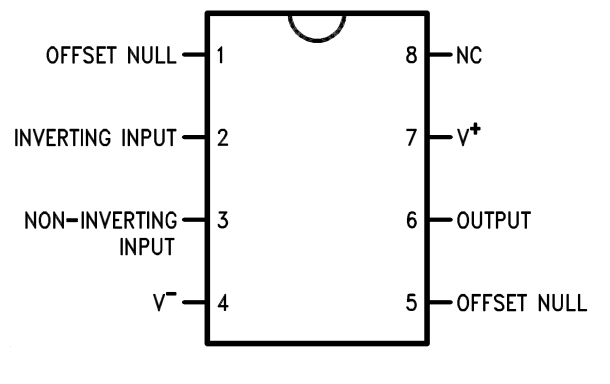
\includegraphics[width=\columnwidth]{images/lab7_1.png}
    \captionof{figure}{Pinout diagram of the LM741 opamp \cite{nsdata}}
    \label{fig:pin}
    \medskip
\endgroup

\noindent As shown by Figure \ref{fig:pin}, LM741 opamp has 8 pins. Pins 2 and 3 are used for input voltage, while Pin 4 \& 7 are used for supplying the opamp and its components with power, in this case 15V. Pin 6 is used to obtain the output conditioned by the opamp. Pins 1, 5, and 8 were not used for this lab. 

\noindent The table below summarizes the instruments used to build the circuits in this experiment.

\begingroup
    \medskip
\centering
\def\arraystretch{1.5}
\begin{tabular}{ll}
\toprule
Item & Quantity \\
\midrule
LM741 Op-Amp & 3 \\
Dual Output Power Supply & 1 \\
1K$\ohm$ Resistors & 3 \\
5.1K$\ohm$ Resistors & 3 \\
10K$\ohm$ Resistors & 3 \\
Oscilloscope & 1 \\
AC Function Generator & 1 \\
Solid-Core Wires & Various Lengths \\
Wire Stripper & 1 \\
\bottomrule
\end{tabular}
\captionof{figure}{Tabulation of the equipment and materials used for this experiment}
\label{fig:table}
    \medskip
\endgroup

\section{Experimental Set-up}

\subsection{Inverting Amplifier}
\noindent The inverting amplifier inverts and amplifies the input signal. The circuit aimed to achieve a gain of -10.

\begingroup
    \centering
    \medskip
    %width=\columnwidth
    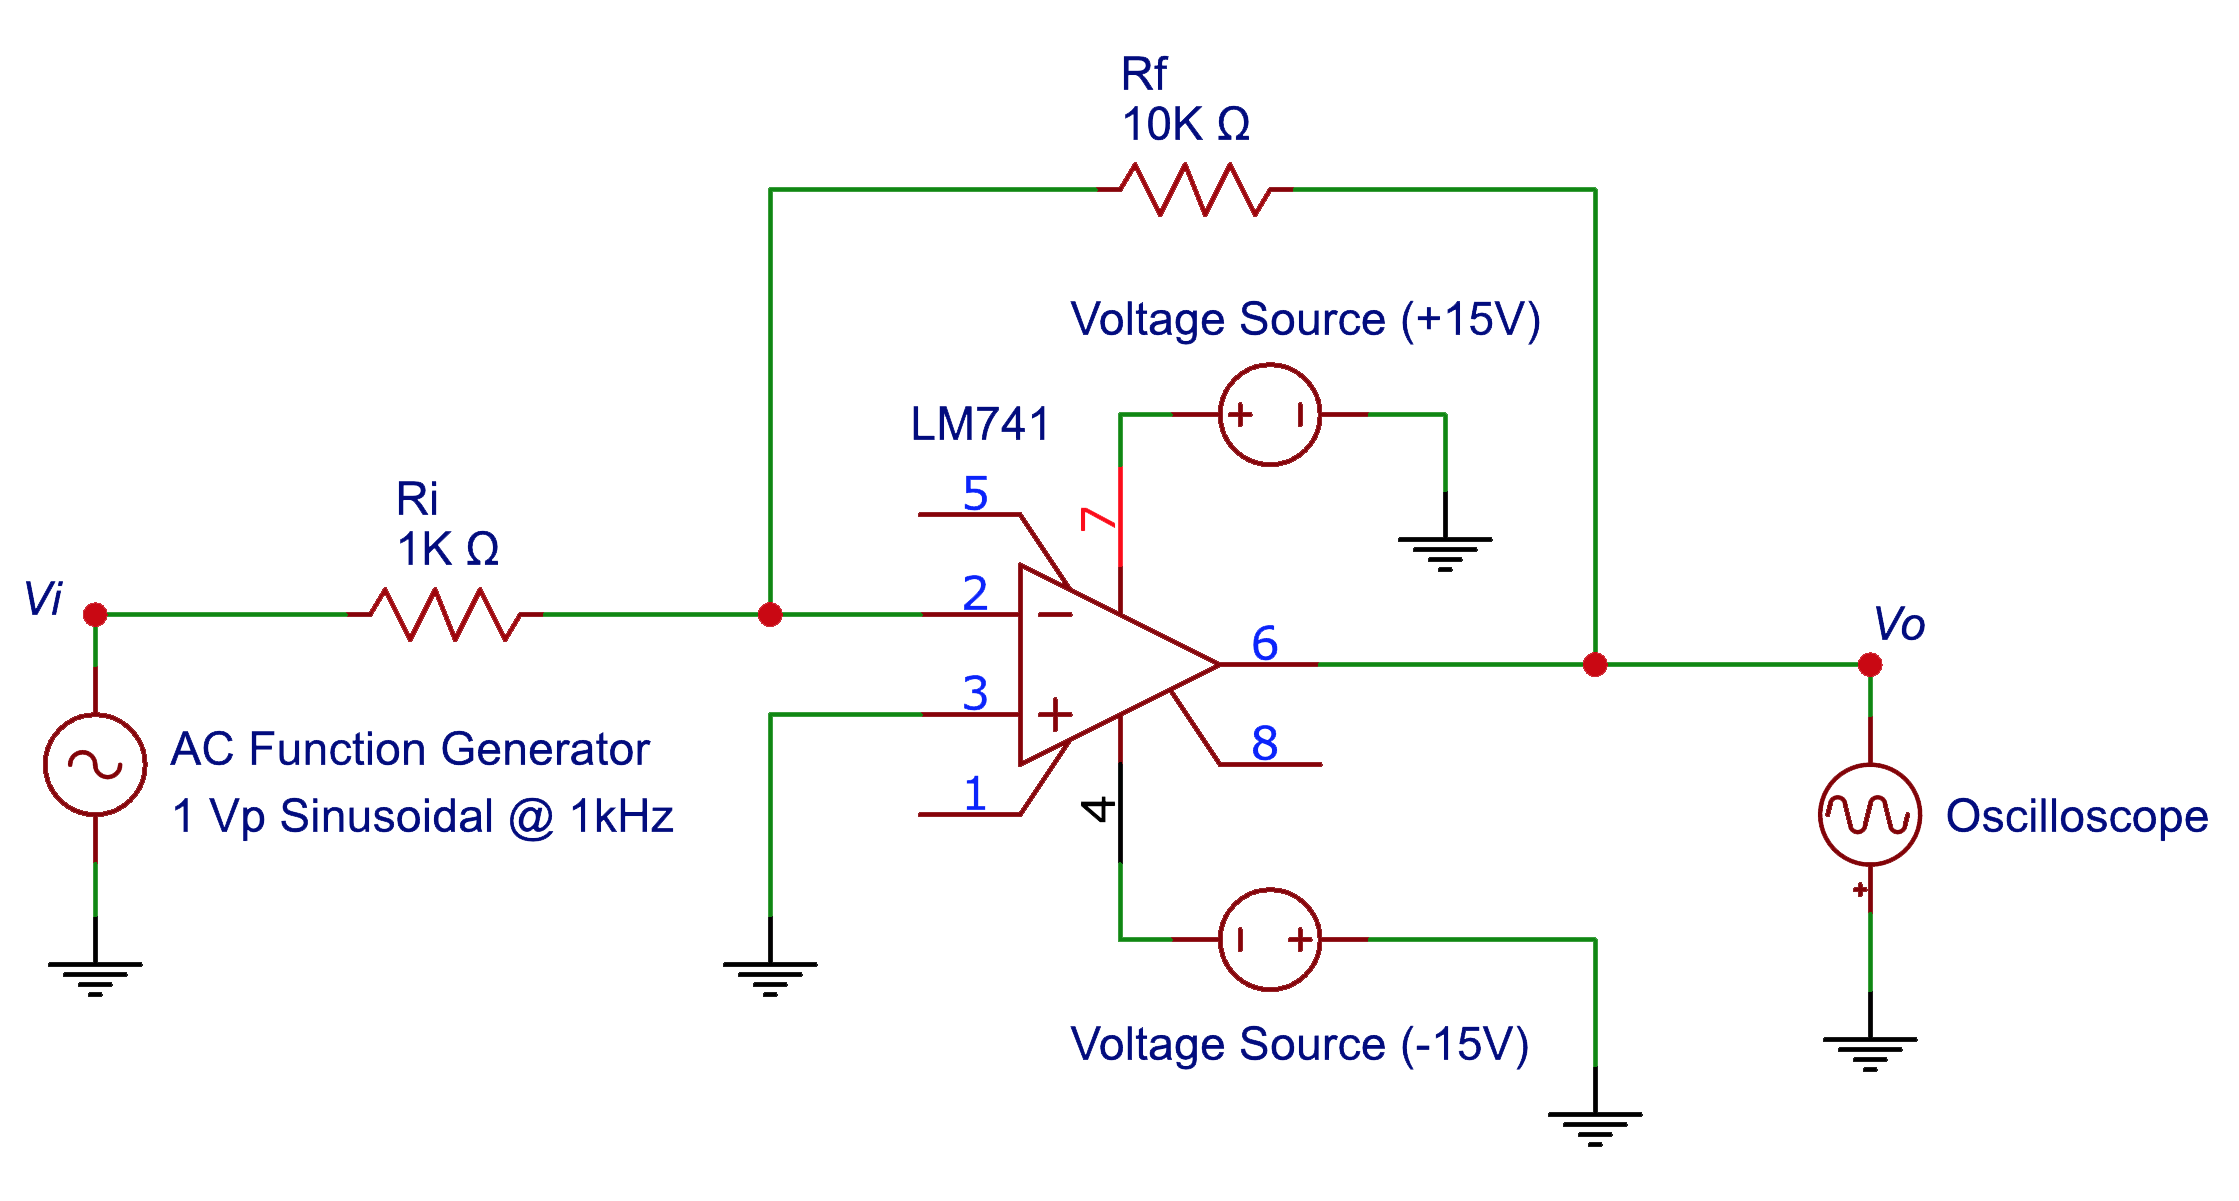
\includegraphics[width=\columnwidth]{images/lab7_inverting.png}
    \captionof{figure}{Schematics of the inverting amplifier circuit built}
    \label{fig:inv_diagram}
    \medskip
\endgroup

\noindent Following the schematic above (Figure \ref{fig:inv_diagram}), the circuit was prototyped on a breadboard. The positive (V+) and negative (V-) power supply terminals were attached to the appropriate power rails on the breadboard, which were then wired to Pins 7 and 4, respectively. The power supplied was +15V and -15V. The non-inverting input was grounded, as $R_p$ was selected to be 0$\ohm$. The output pin 6 was connected to the inverting input (pin 2) with a 10K$\ohm$ resistor, while the input voltage was also supplied to pin 2 through a 1K$\ohm$ resistor.

\begin{equation}
Gain = \frac{V_o}{V_i} = -\frac{10K\ohm}{1K\ohm} = -10
\label{eq:inverting}
\end{equation}


\noindent Once the circuit was reproduced as shown in  Figure \ref{fig:inv_circ}, the operation of the circuit was verified with a 1V input signal with a frequency of 1kHz.

\begingroup
    \centering
    \medskip
    %width=\columnwidth
    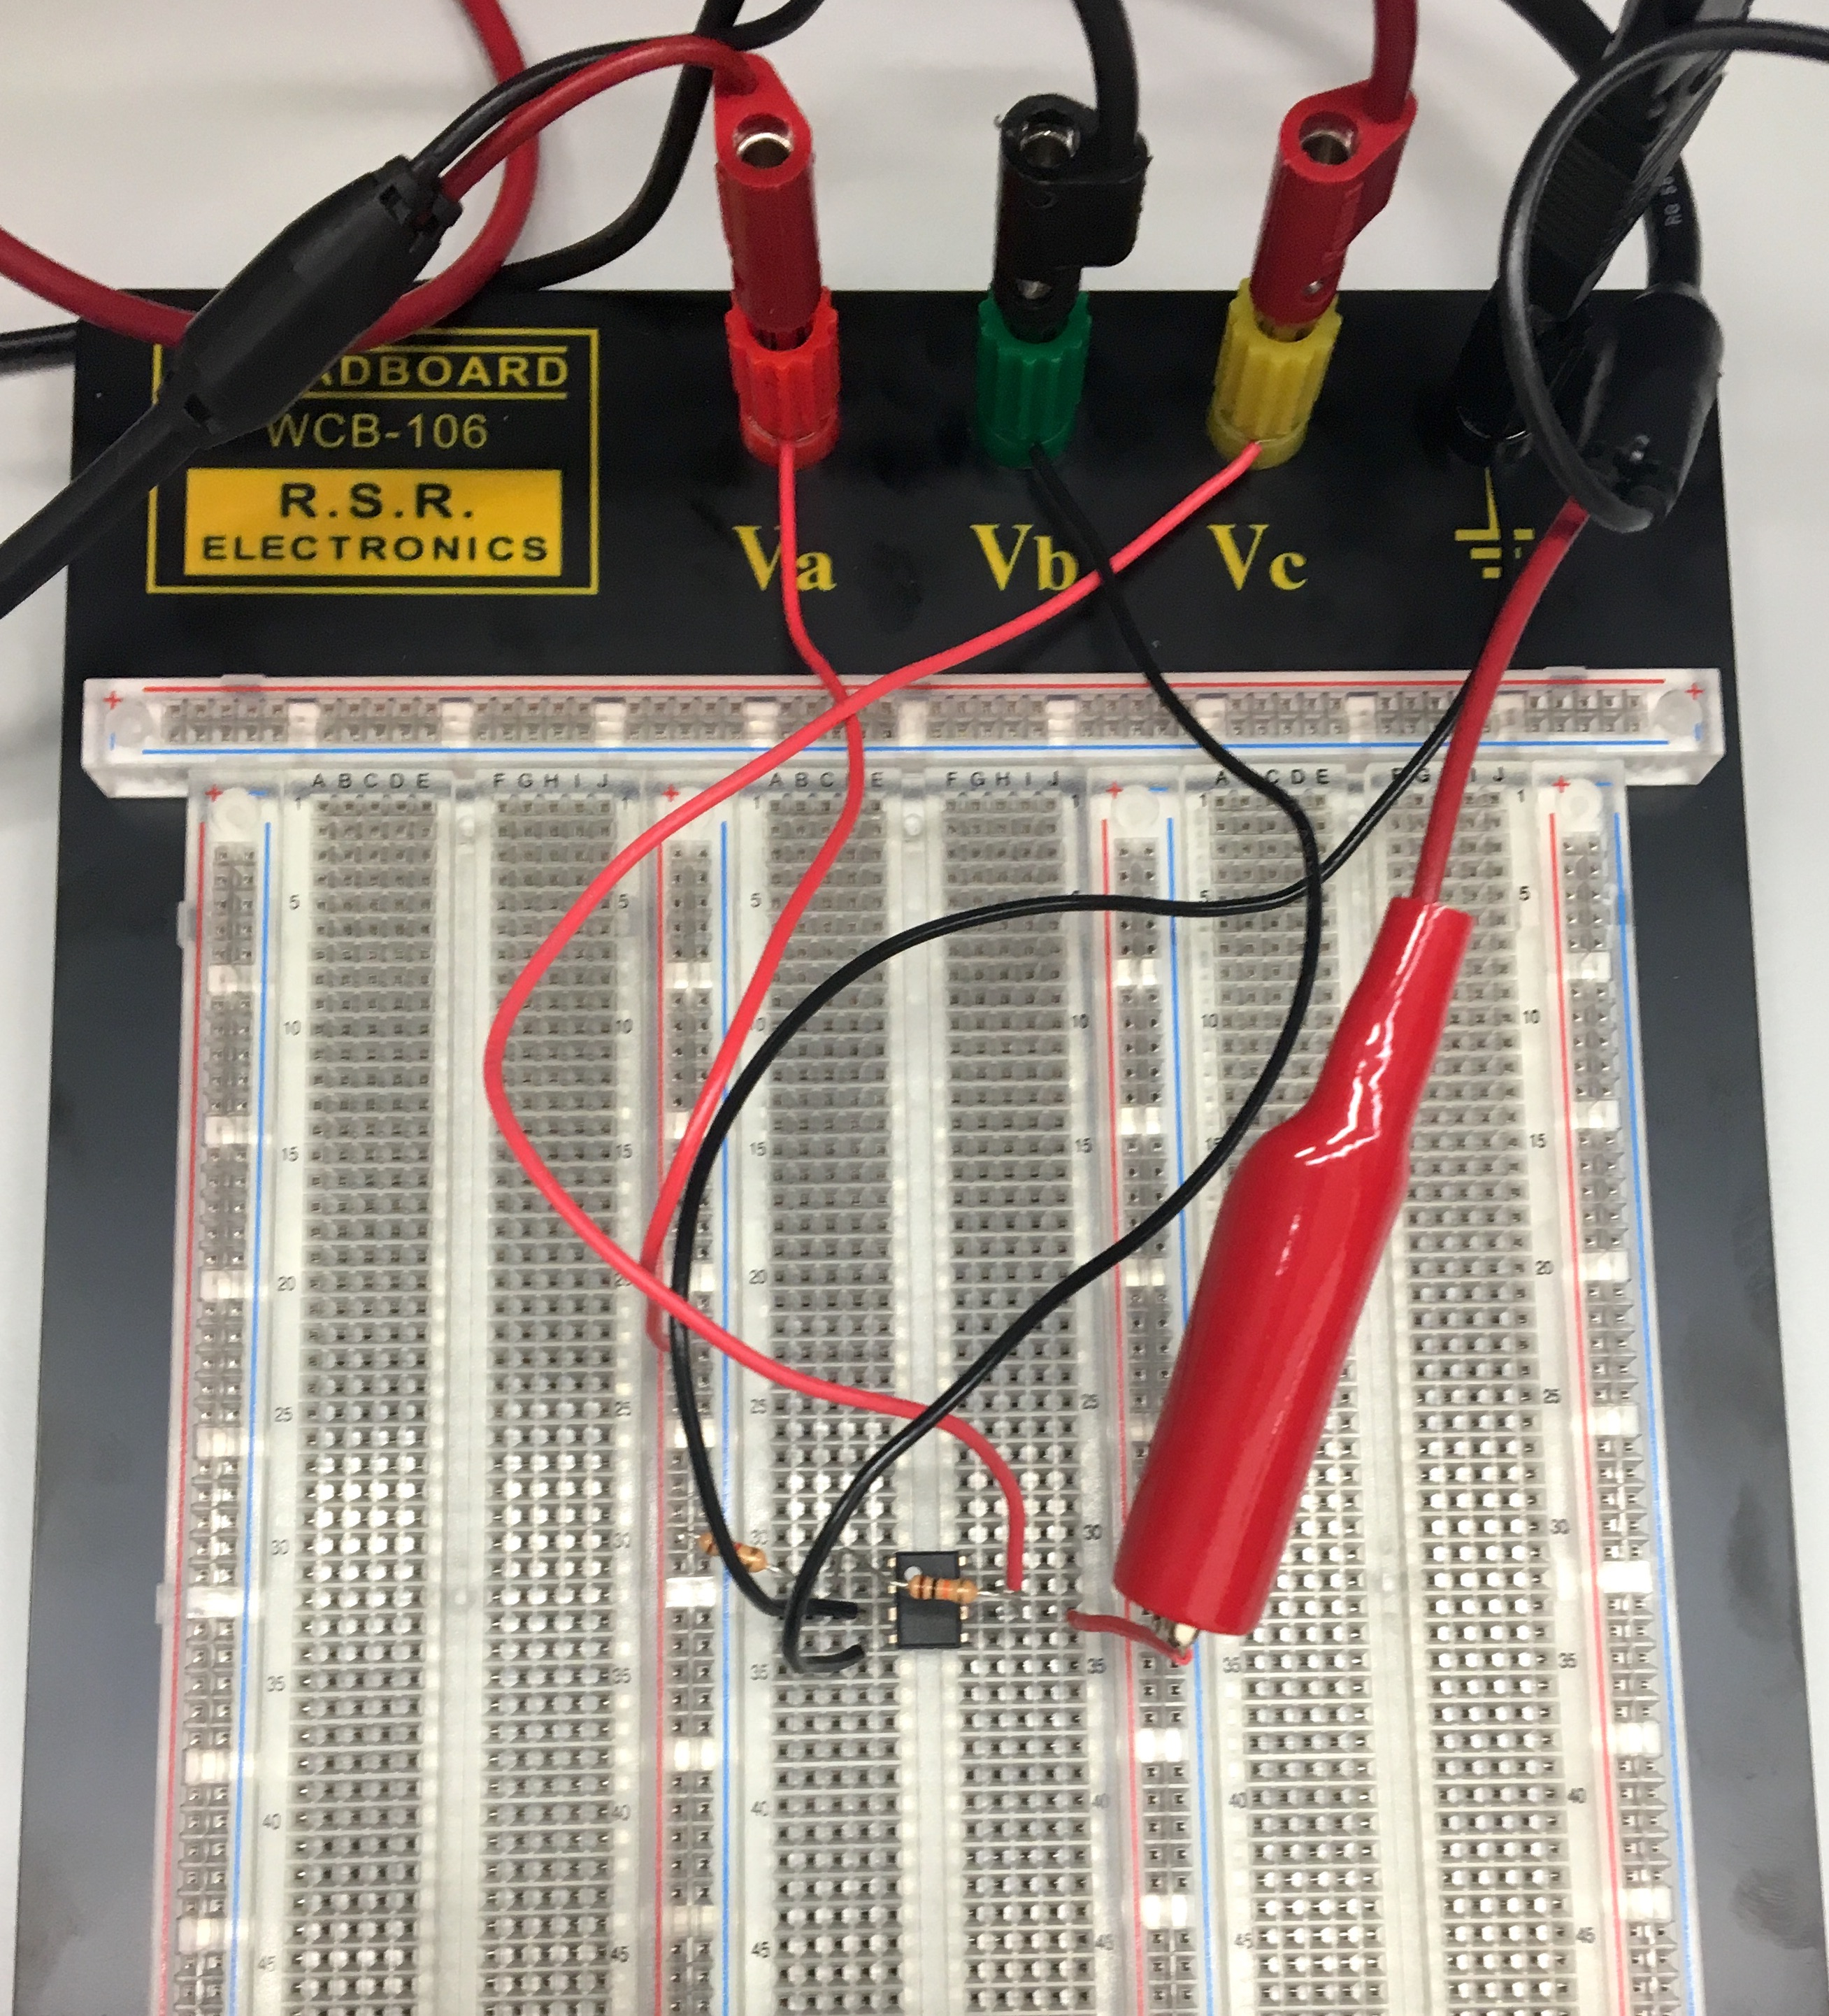
\includegraphics[width=\columnwidth]{images/lab7_inverting_circuit.jpg}
    \captionof{figure}{The inverting amplifier circuit built based on the schematics}
    \label{fig:inv_circ}
    \medskip
\endgroup




                                %%%%%%%%%%%%% %%%%%%%%%%%%%
                                %%%%%%%%%%%%   %%%%%%%%%%%%    
                                %%%%%%%%%%%     %%%%%%%%%%%
                                %%%%%%%%%%       %%%%%%%%%%    
                                
\subsection{Non-Inverting Amplifier}
\noindent The non-inverting amplifier simply amplifies the input signal without inverting it. The circuit aimed to achieve a gain of 11.

\begingroup
    \centering
    \medskip
    %width=\columnwidth
    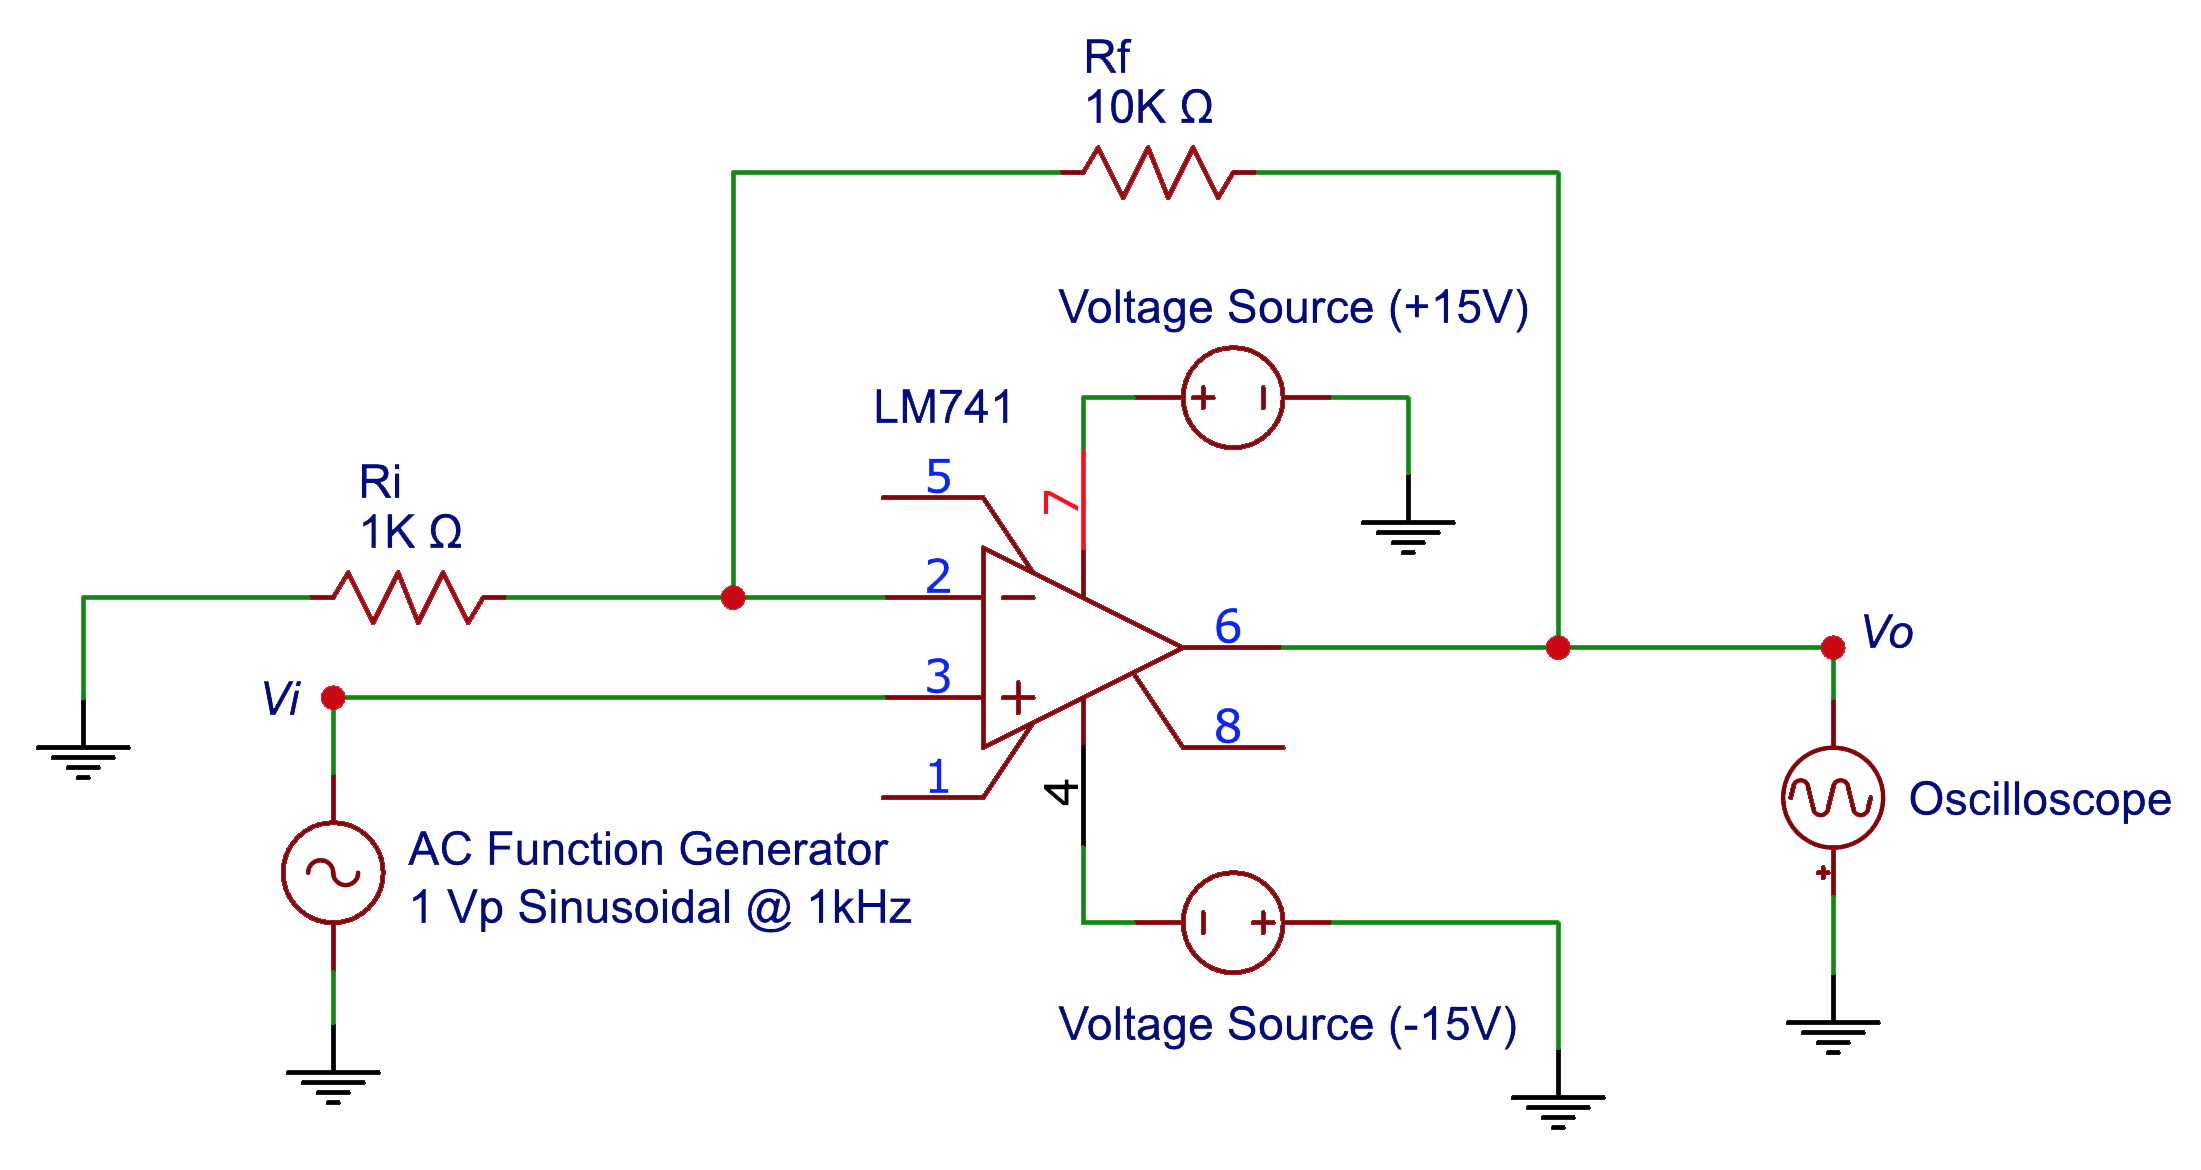
\includegraphics[width=\columnwidth]{images/lab7_non-inverting.png}
    \captionof{figure}{Schematics of the non-inverting amplifier circuit built}
    \label{fig:non_inv_diagram}
    \medskip
\endgroup

\noindent Following the schematic above (Figure \ref{fig:non_inv_diagram}), the circuit was prototyped on a breadboard beside the inverting amplifier. The non-inverting input (pin 3) was directly fed the input voltage. The output (pin 6) was connected to the inverting input (pin 2) with a 10K$\ohm$ resistor. The inverting input was also grounded with a 1K$\ohm$ resistor. Power was supplied as in the previous configuration.

\begin{equation}
Gain = \frac{V_o}{V_i} = 1 + \frac{10K \ohm}{1K \ohm} = 11
\label{eq:non-inverting}
\end{equation}

\noindent Once the circuit was reproduced as shown in  Figure \ref{fig:non-inv_circ}, the operation of the circuit was verified with a 1V input signal with a frequency of 1kHz.

\begingroup
    \centering
    \medskip
    %width=\columnwidth
    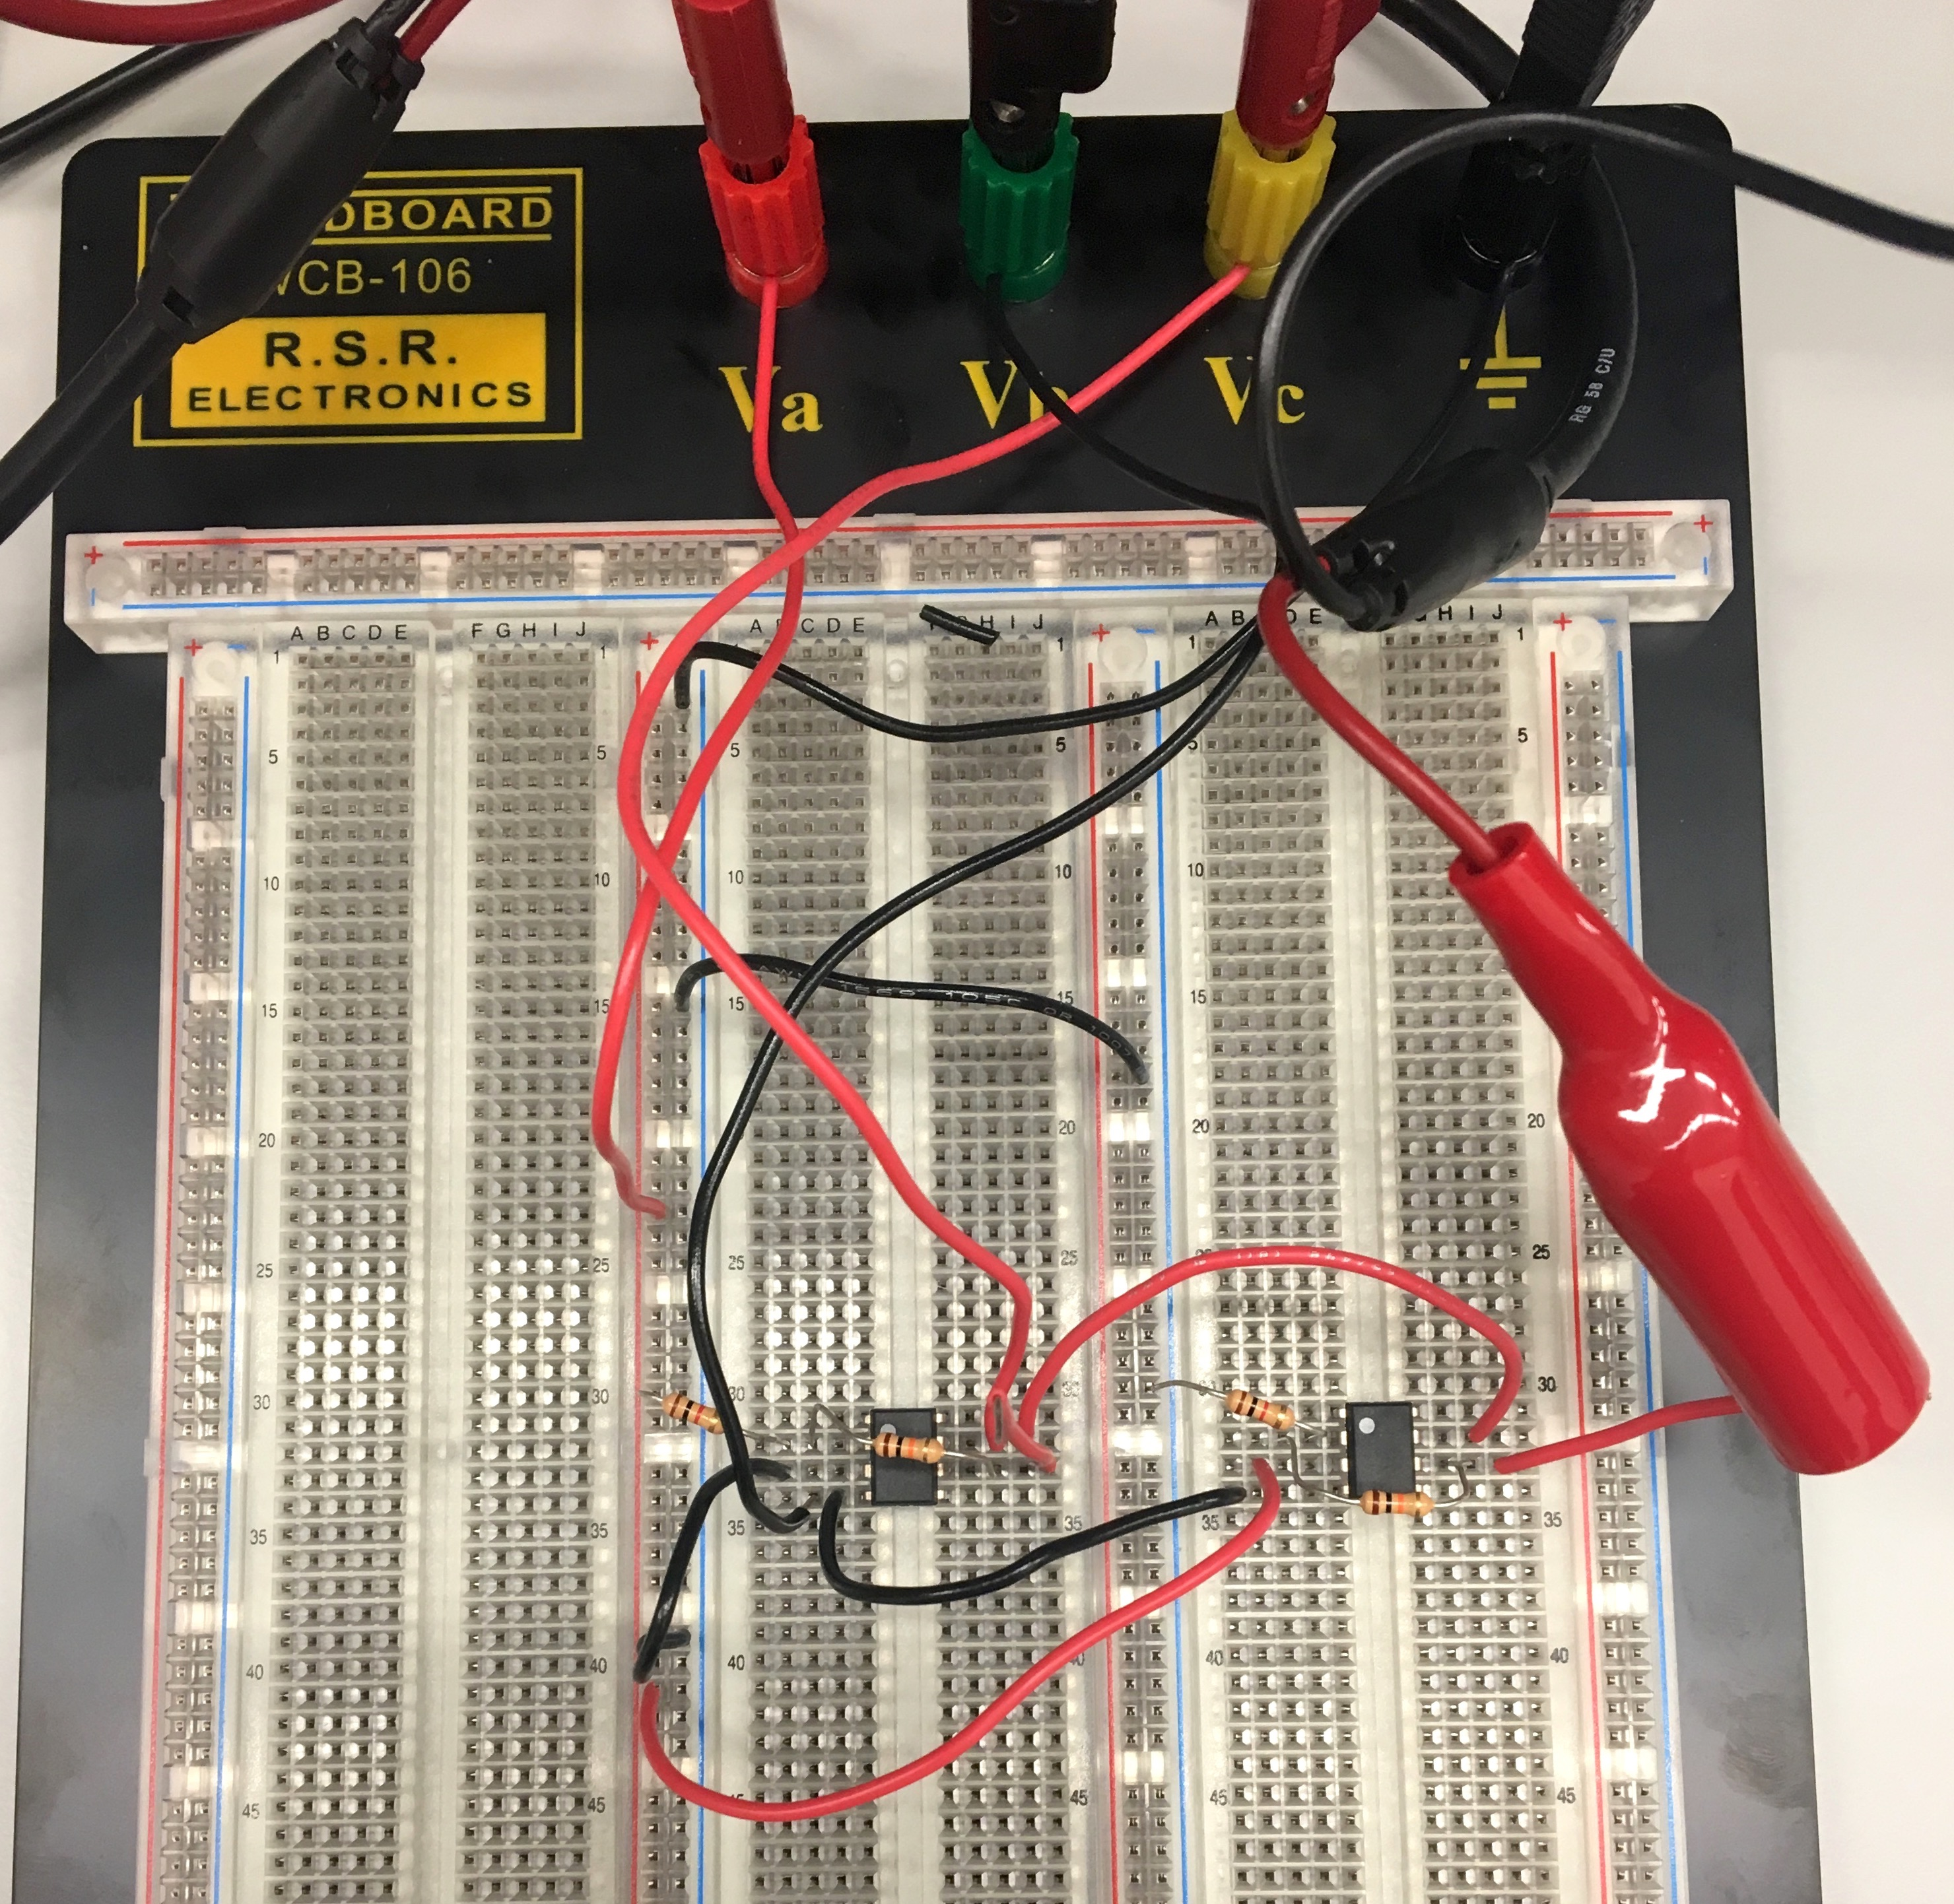
\includegraphics[width=\columnwidth]{images/lab7_non_inverting_circuit.jpg}
    \captionof{figure}{The non-inverting amplifier circuit built on the right side of the inverting amplifier circuit}
    \label{fig:non-inv_circ}
    \medskip
\endgroup




                                %%%%%%%%%%%%% %%%%%%%%%%%%%
                                %%%%%%%%%%%%   %%%%%%%%%%%%    
                                %%%%%%%%%%%     %%%%%%%%%%%
                                %%%%%%%%%%       %%%%%%%%%%    
                                

\subsection{Cascading Amplifier}
\noindent The cascading amplifier works to magnify the output voltage by daisy chaining multiple amplifiers together as shown in Figure \ref{fig:cascade_diagram}, where pin 6 of the top circuit is ported to pin 3 of the bottom circuit.

\begingroup
    \centering
    \medskip
    %width=\columnwidth
    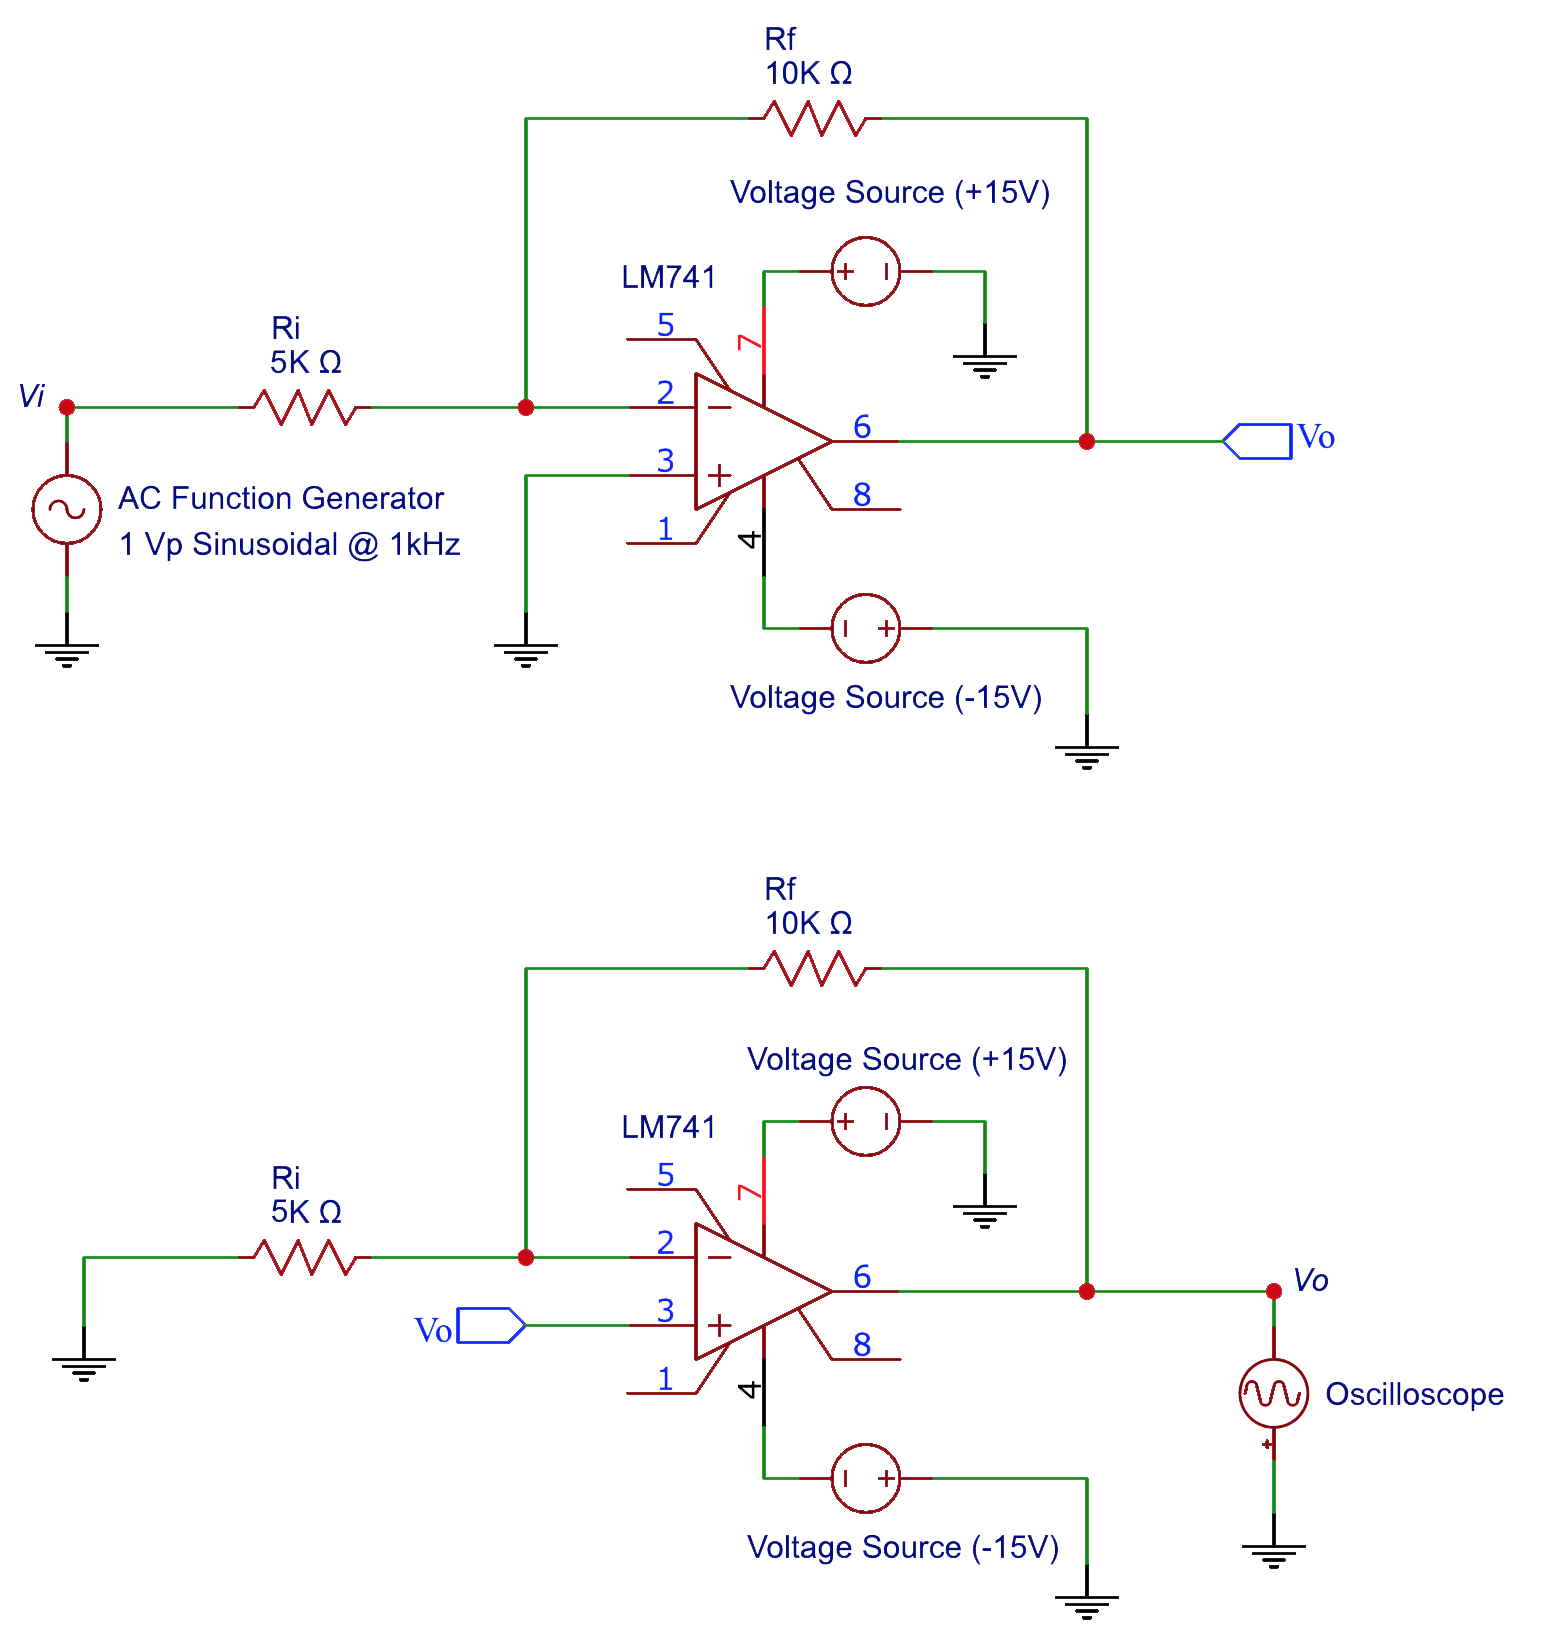
\includegraphics[width=\columnwidth]{images/lab7_cascading.png}
    \captionof{figure}{Schematics of the cascaded circuit built using a non-inverting and an inverting amplifier circuit}
    \label{fig:cascade_diagram}
    \medskip
\endgroup

The circuit aimed to achieve a gain of 6, 2 from the inverting and 3 from the non-inverting. In order to determine the resistors needed, equations \ref{eq:inverting} and \ref{eq:non-inverting} were combined to produce equation \ref{eq:cascading}. $R_f$ was selected to be $10K\ohm$ and $R_i$ as $5K\ohm$ to minimize the changes made to the circuitry.

\begin{equation}
Gain = \abs(\frac{R_f}{R_i}) * (\frac{R_f}{R_i} + 1) = \frac{10K\ohm}{5K\ohm} * (\frac{10K\ohm}{5K\ohm} + 1) =  6
\label{eq:cascading}
\end{equation}

\bigskip
    
\noindent Using Figure \ref{fig:cascade_diagram}, the output of the inverting amplifier (pin 6) was fed into the non-inverting input (pin 3) of the non-inverting amplifier. Next, the inverting input (pin 2) of the non-inverting amplifier was connected to the common ground. The original $R_i$, with its value of $1K\ohm$, was replaced with a $5.1K\ohm$ resistor on both amplifiers, as it was the closest appropriate resistor to $5K\ohm$. After ensuring that both amplifiers shared the same source voltages (+15V at pin 7 and -15V at pin 4) and a common ground, an input signal of 1V input and a frequency of 1kHz was used to verify operation. The output signal was measured by connecting pin 6 of the non-inverting amplifier to the oscilloscope as shown in Figure \ref{fig:cascade_circ}.

\begingroup
    \centering
    \bigskip
    %width=\columnwidth
    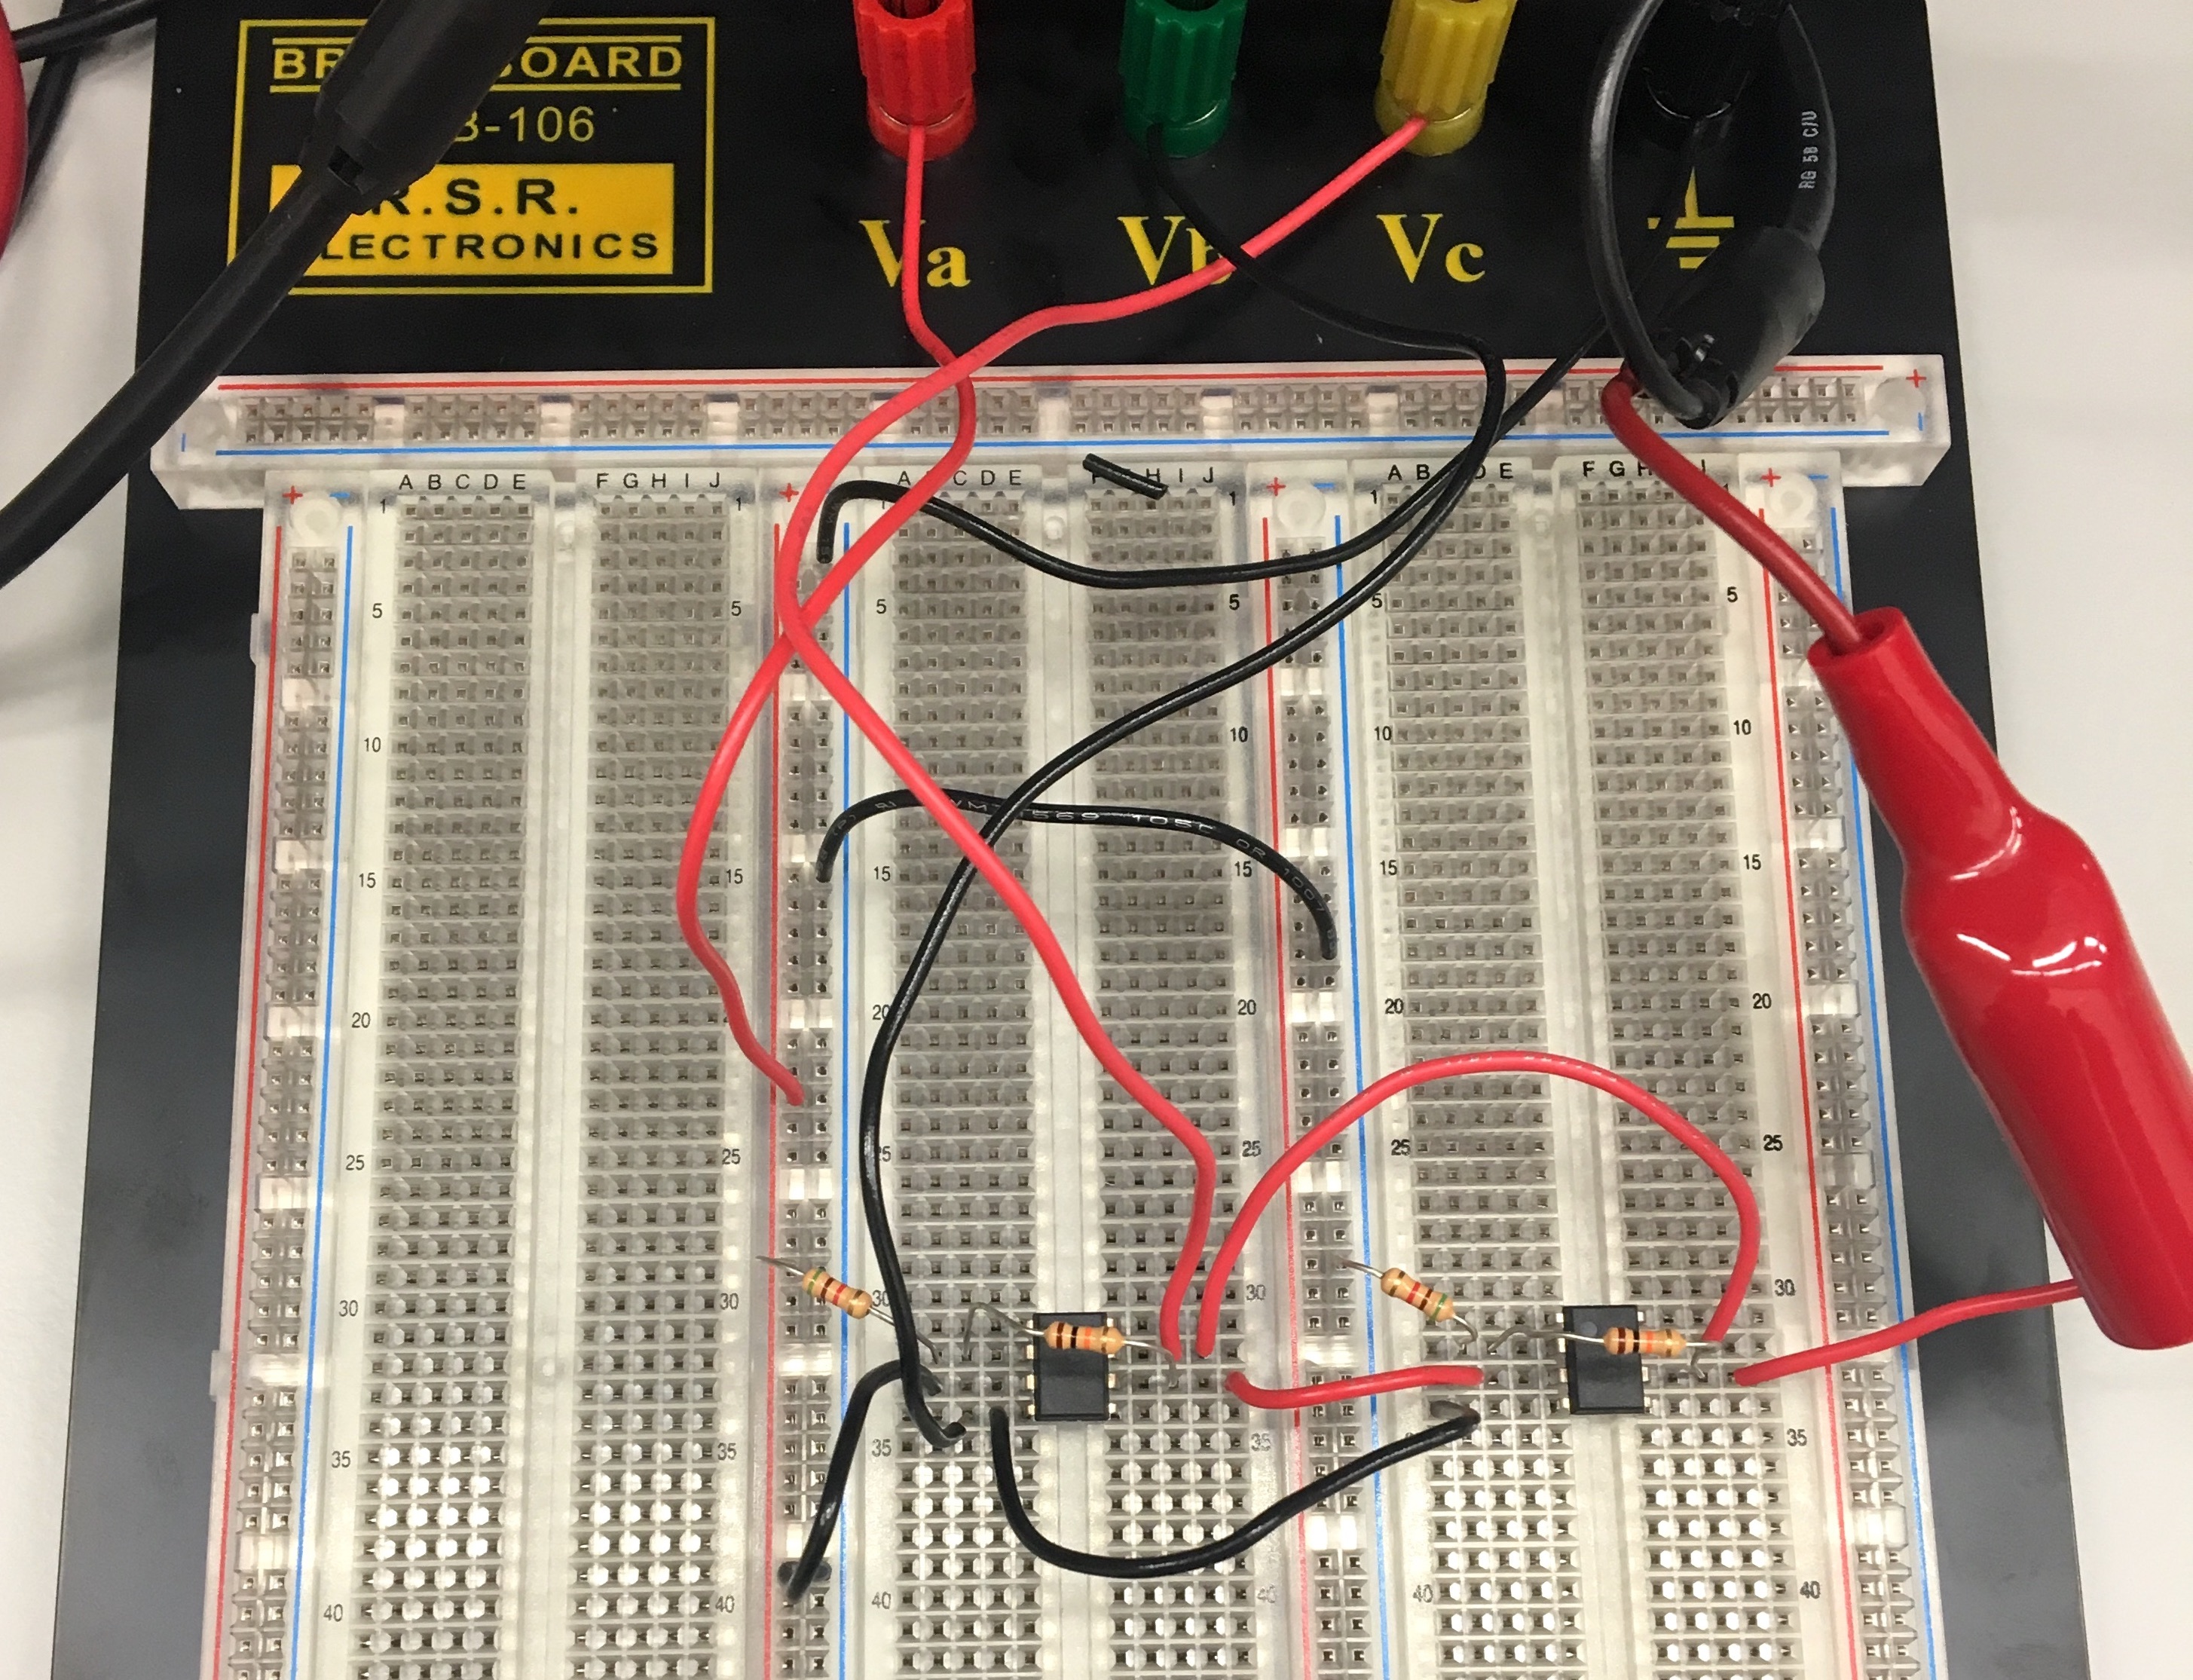
\includegraphics[width=\columnwidth]{images/lab7_cascading_circuit.jpg}
    \captionof{figure}{The cascading amplifier circuit built by combining previously built inverting and non-inverting amplifier circuits}
    \label{fig:cascade_circ}
    \medskip
\endgroup

\subsection{Summing Amplifier}
\noindent The summing amplifier sums a ratio of the input voltages; in the case where all the resistors are equal, the equation is as follows:

\begin{equation}
V_o = -(V_1+V_2)
\label{eq:summing}
\end{equation}

\begingroup
    \centering
    \medskip
    %width=\columnwidth
    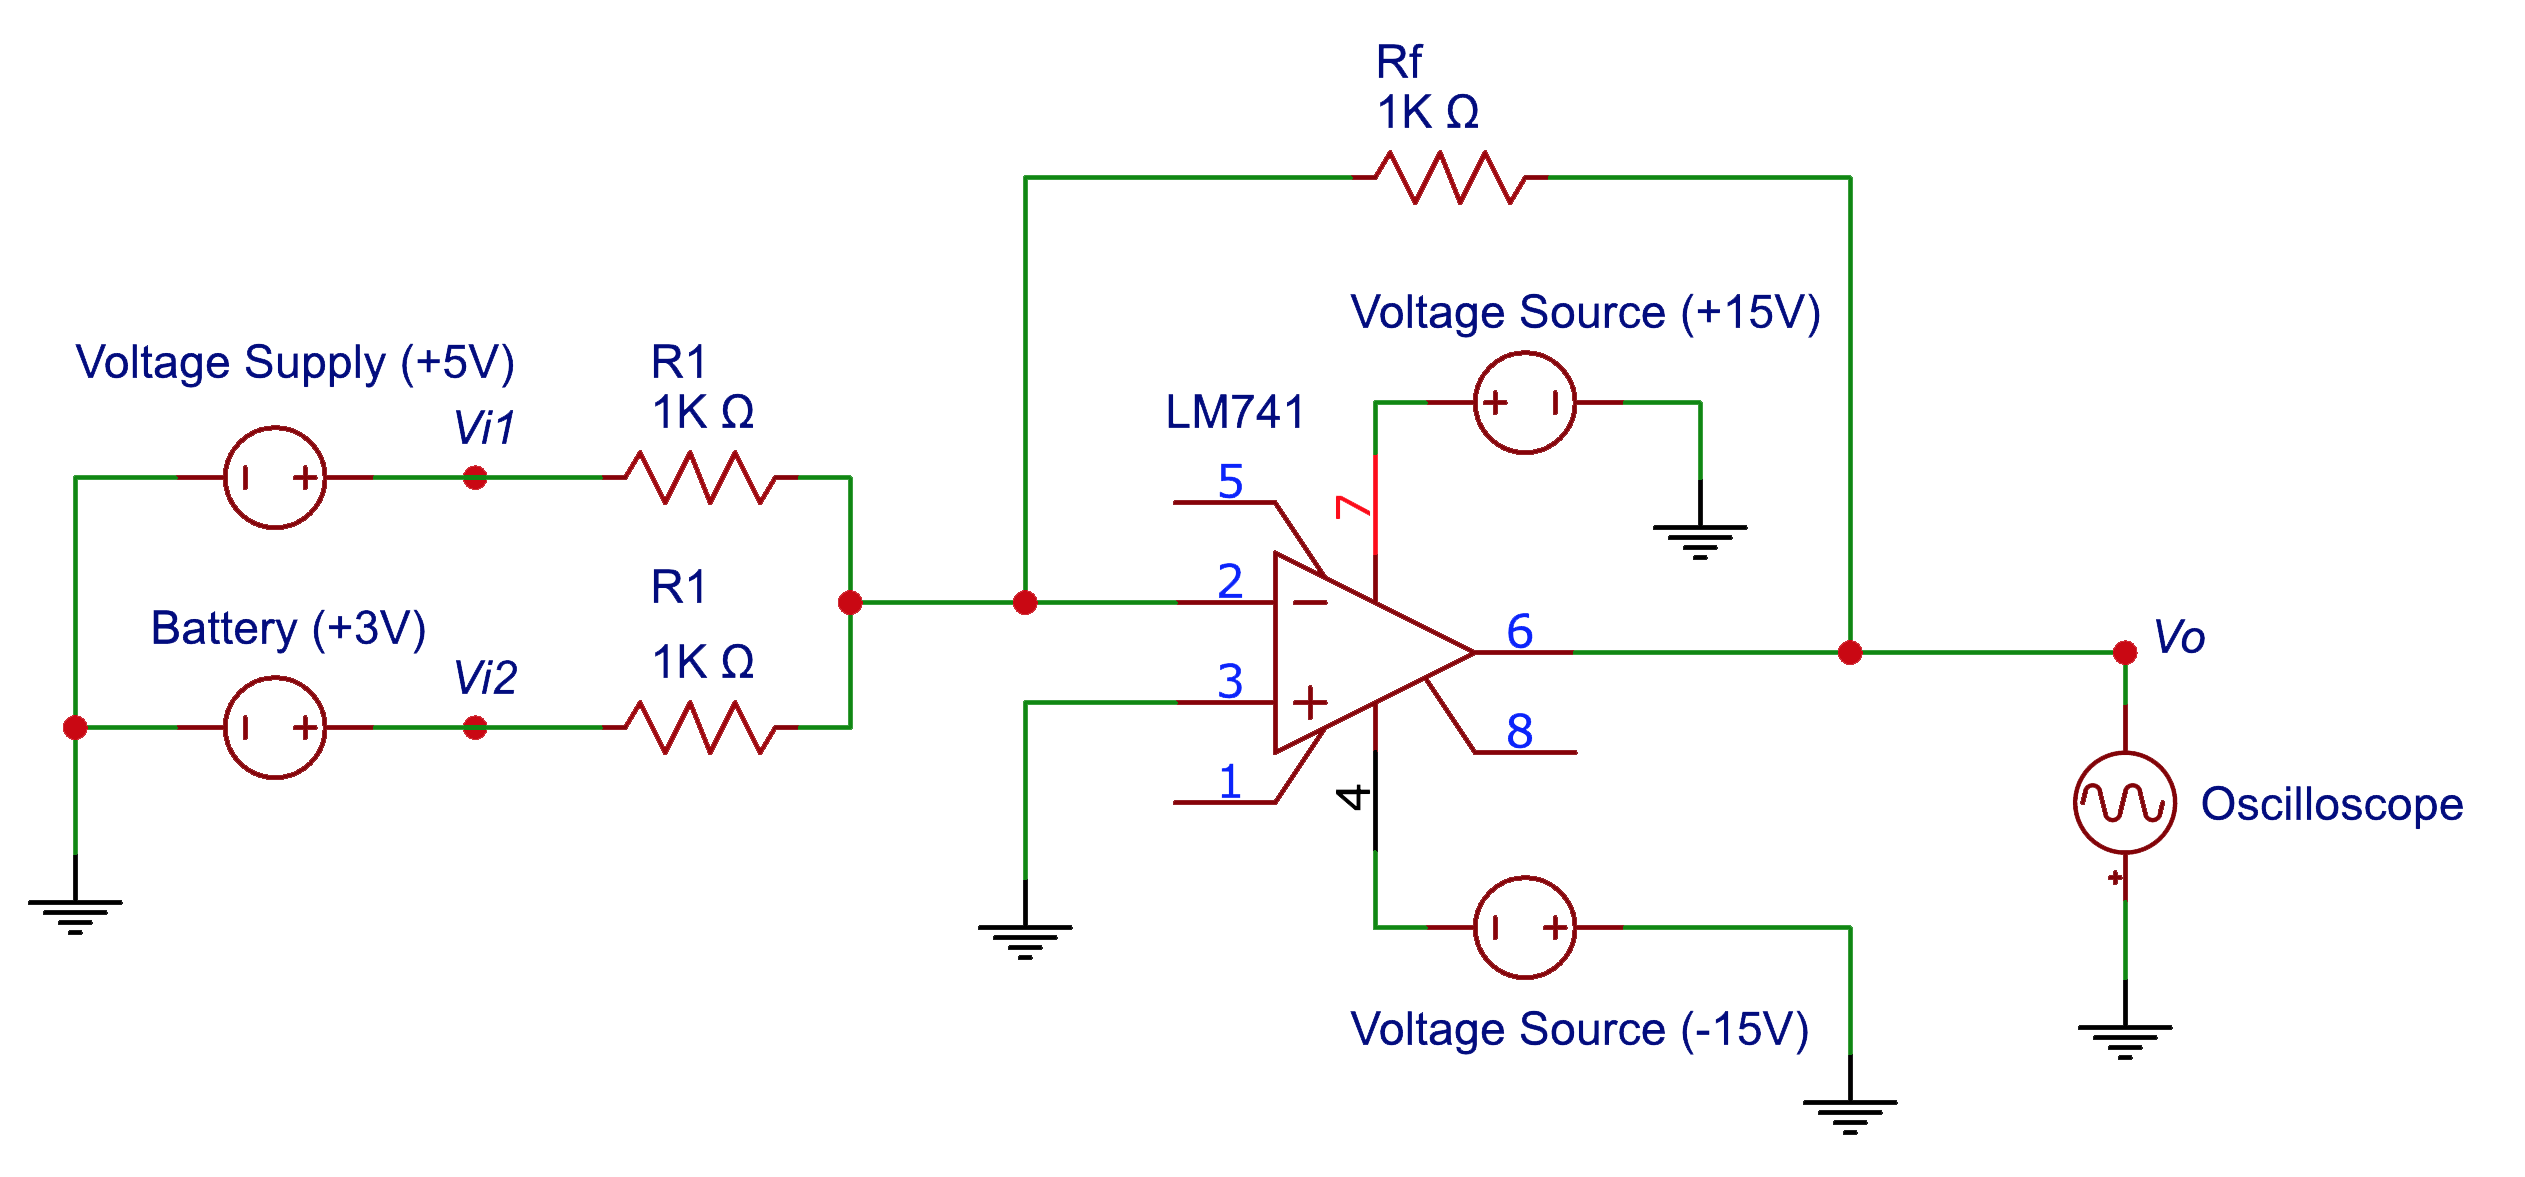
\includegraphics[width=\columnwidth]{images/lab7_summing.png}
    \captionof{figure}{Schematics of the summing amplifier circuit built}
    \label{fig:summing}
    \medskip
\endgroup

\noindent With Figure \ref{fig:summing} as reference, +15V voltage source was connected to pin 7 and -15V voltage source was connected to pin 4. The first input voltage, +5V, was connected to the inverting input (pin 2) through a $1K\ohm$ resistor, while the second input voltage, batteries providing +3V, were connected to the non-inverting input (pin 5) through a $1K\ohm$ resistor. Finally, the output voltage (pin 6) was fed back into the inverting input (pin 2) through another $1K\ohm$ resistor as shown in Figure \ref{fig:summing_circ}.

\begingroup
    \centering
    \medskip
    %width=\columnwidth
    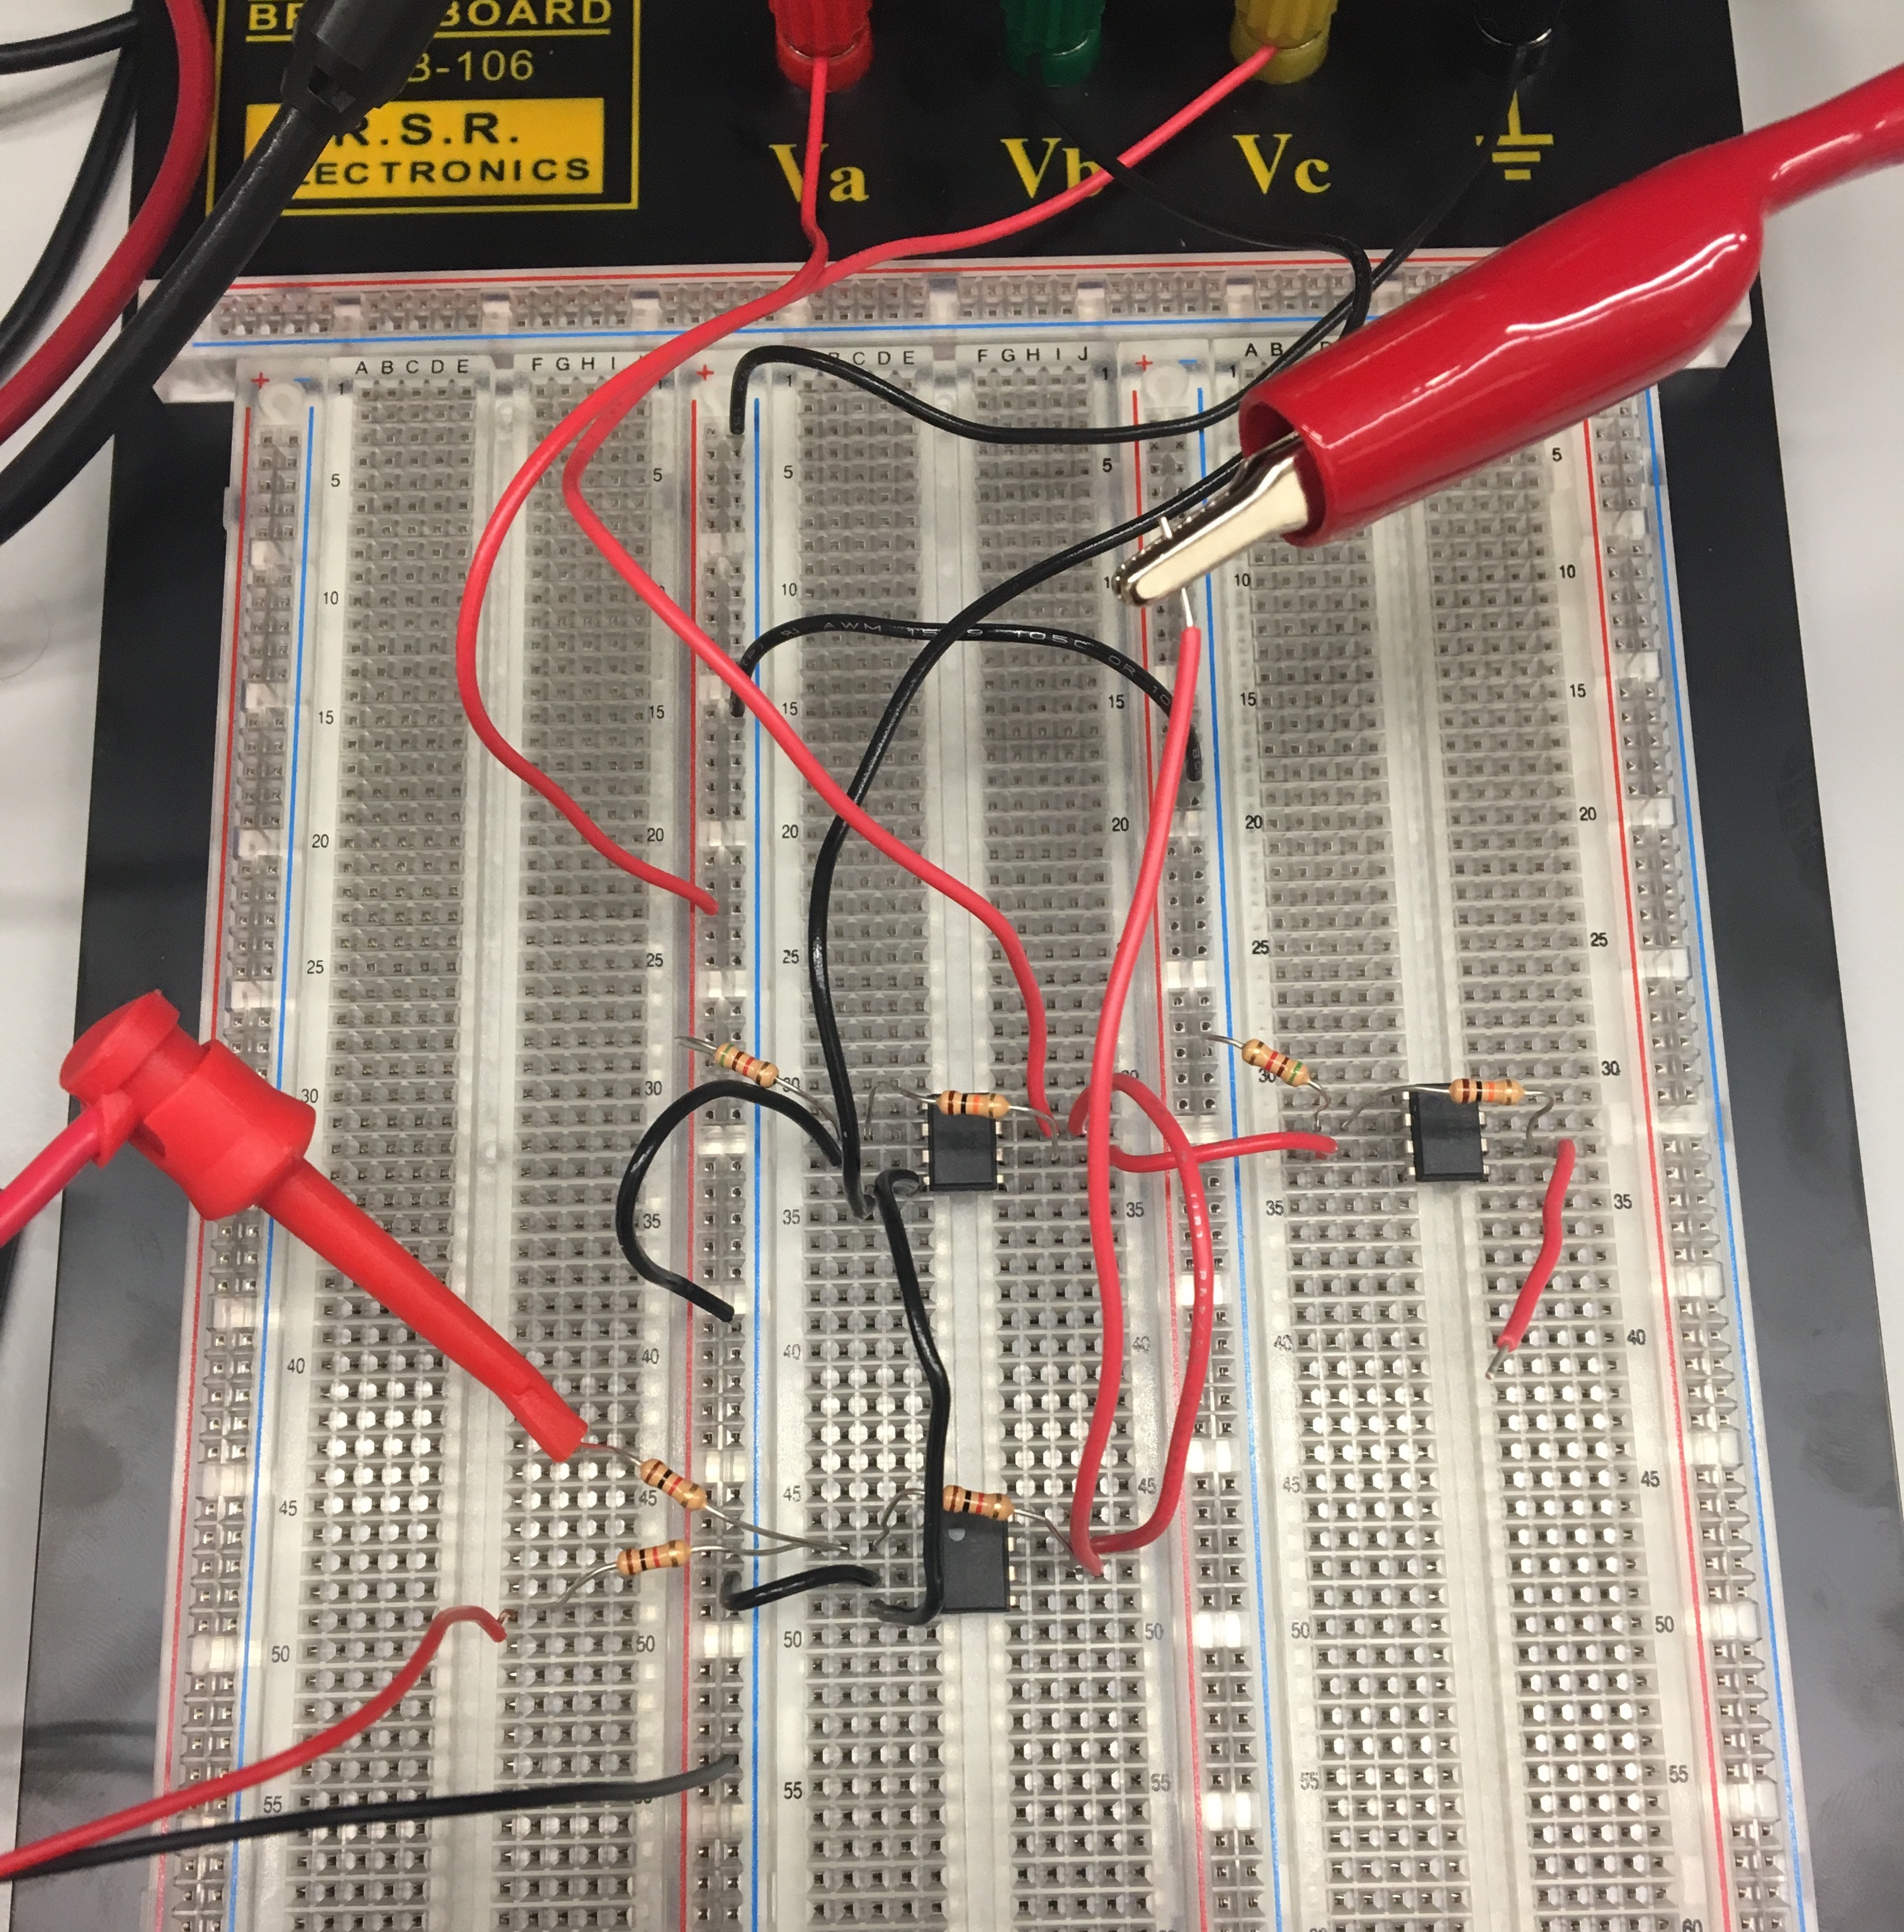
\includegraphics[width=\columnwidth]{images/lab7_summing_circuit.jpg}
    \captionof{figure}{The summing amplifier circuit built. The red and black cables on the extreme left bottom corner are connected to the battery voltage source.}
    \label{fig:summing_circ}
    \medskip
\endgroup

\section{Results and Discussion}
\noindent All configurations operated as expected and the results were recorded in the the table below:

\begingroup
\bigskip
\centering
\def\arraystretch{1.5}
\begin{tabular}{lccc}
\toprule
Amplifier Type & Input(s) (V) & Output (V) & Gain \\
\midrule
Inverting Amplifier & 1 & 10 & 10\\
Non-Inverting Amplifier & 1 & 11 & 11\\
Cascading of Amplifiers & 1 & 6 & 6\\
Summing Amplifier & 3 and 5 & 8 & $\frac{8}{3}$ and $\frac{8}{5}$
\bottomrule
\end{tabular}
\captionof{figure}{Tabulation of the measurements for different types of amplifiers}
\label{fig:table}
    \medskip
\endgroup

\noindent The inverting amplifier produced the graph seen in Figure \ref{fig:inverting_osc}, where the output wave (yellow) is seen to lag the input wave (green) by 180 degrees, resulting in an inversion. Counting the divisions, using the values on the top left of the figure, the input signal has an approximate voltage of 1V, while the output voltage has an approximate voltage of 10V; therefore, the gain is 10, as previously calculated.

\begingroup
    \centering
    \medskip
    %width=\columnwidth
    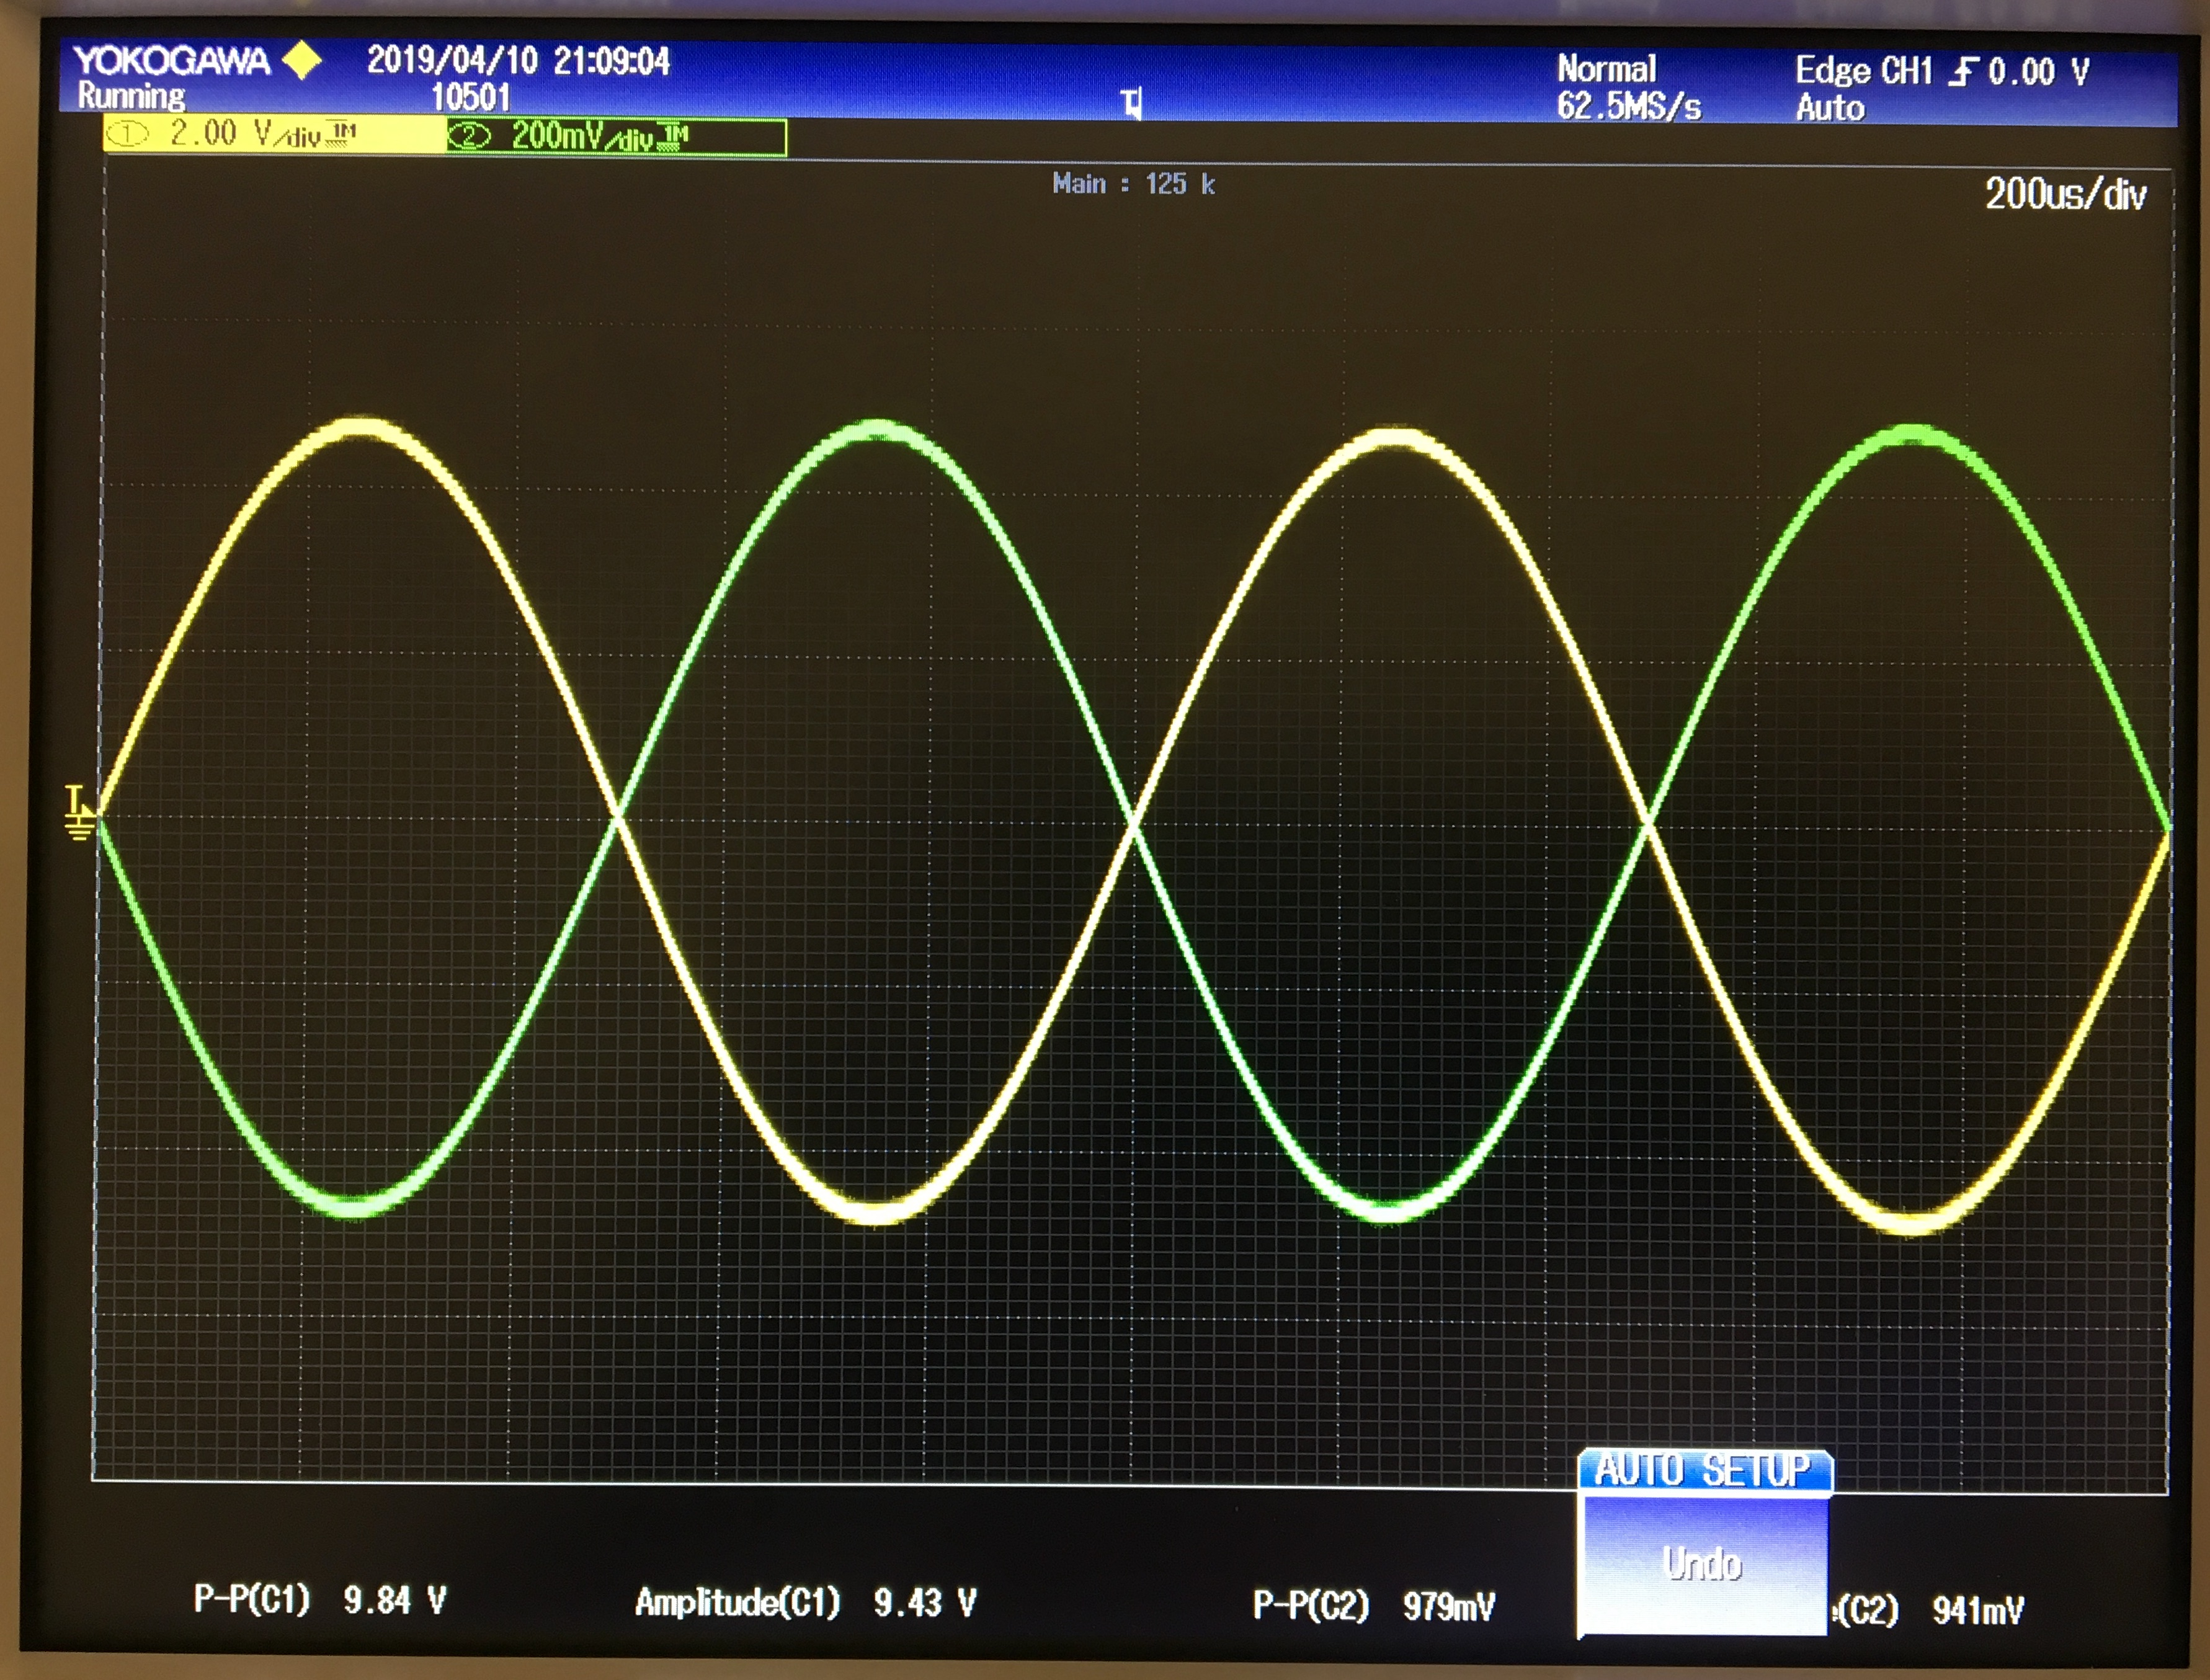
\includegraphics[width=\columnwidth]{images/lab7_inverting_osc.jpg}
    \captionof{figure}{Output of the inverting amplifier}
    \label{fig:inverting_osc}
    \medskip
\endgroup

\noindent The output of the non-inverting amplifier can be seen in Figure \ref{fig:non_inverting_osc}. The input signal has an approximate value of 1V, while the output signal has an approximate value of 11V, leading to the predicted gain of 11. 

\begingroup
    \centering
    \medskip
    %width=\columnwidth
    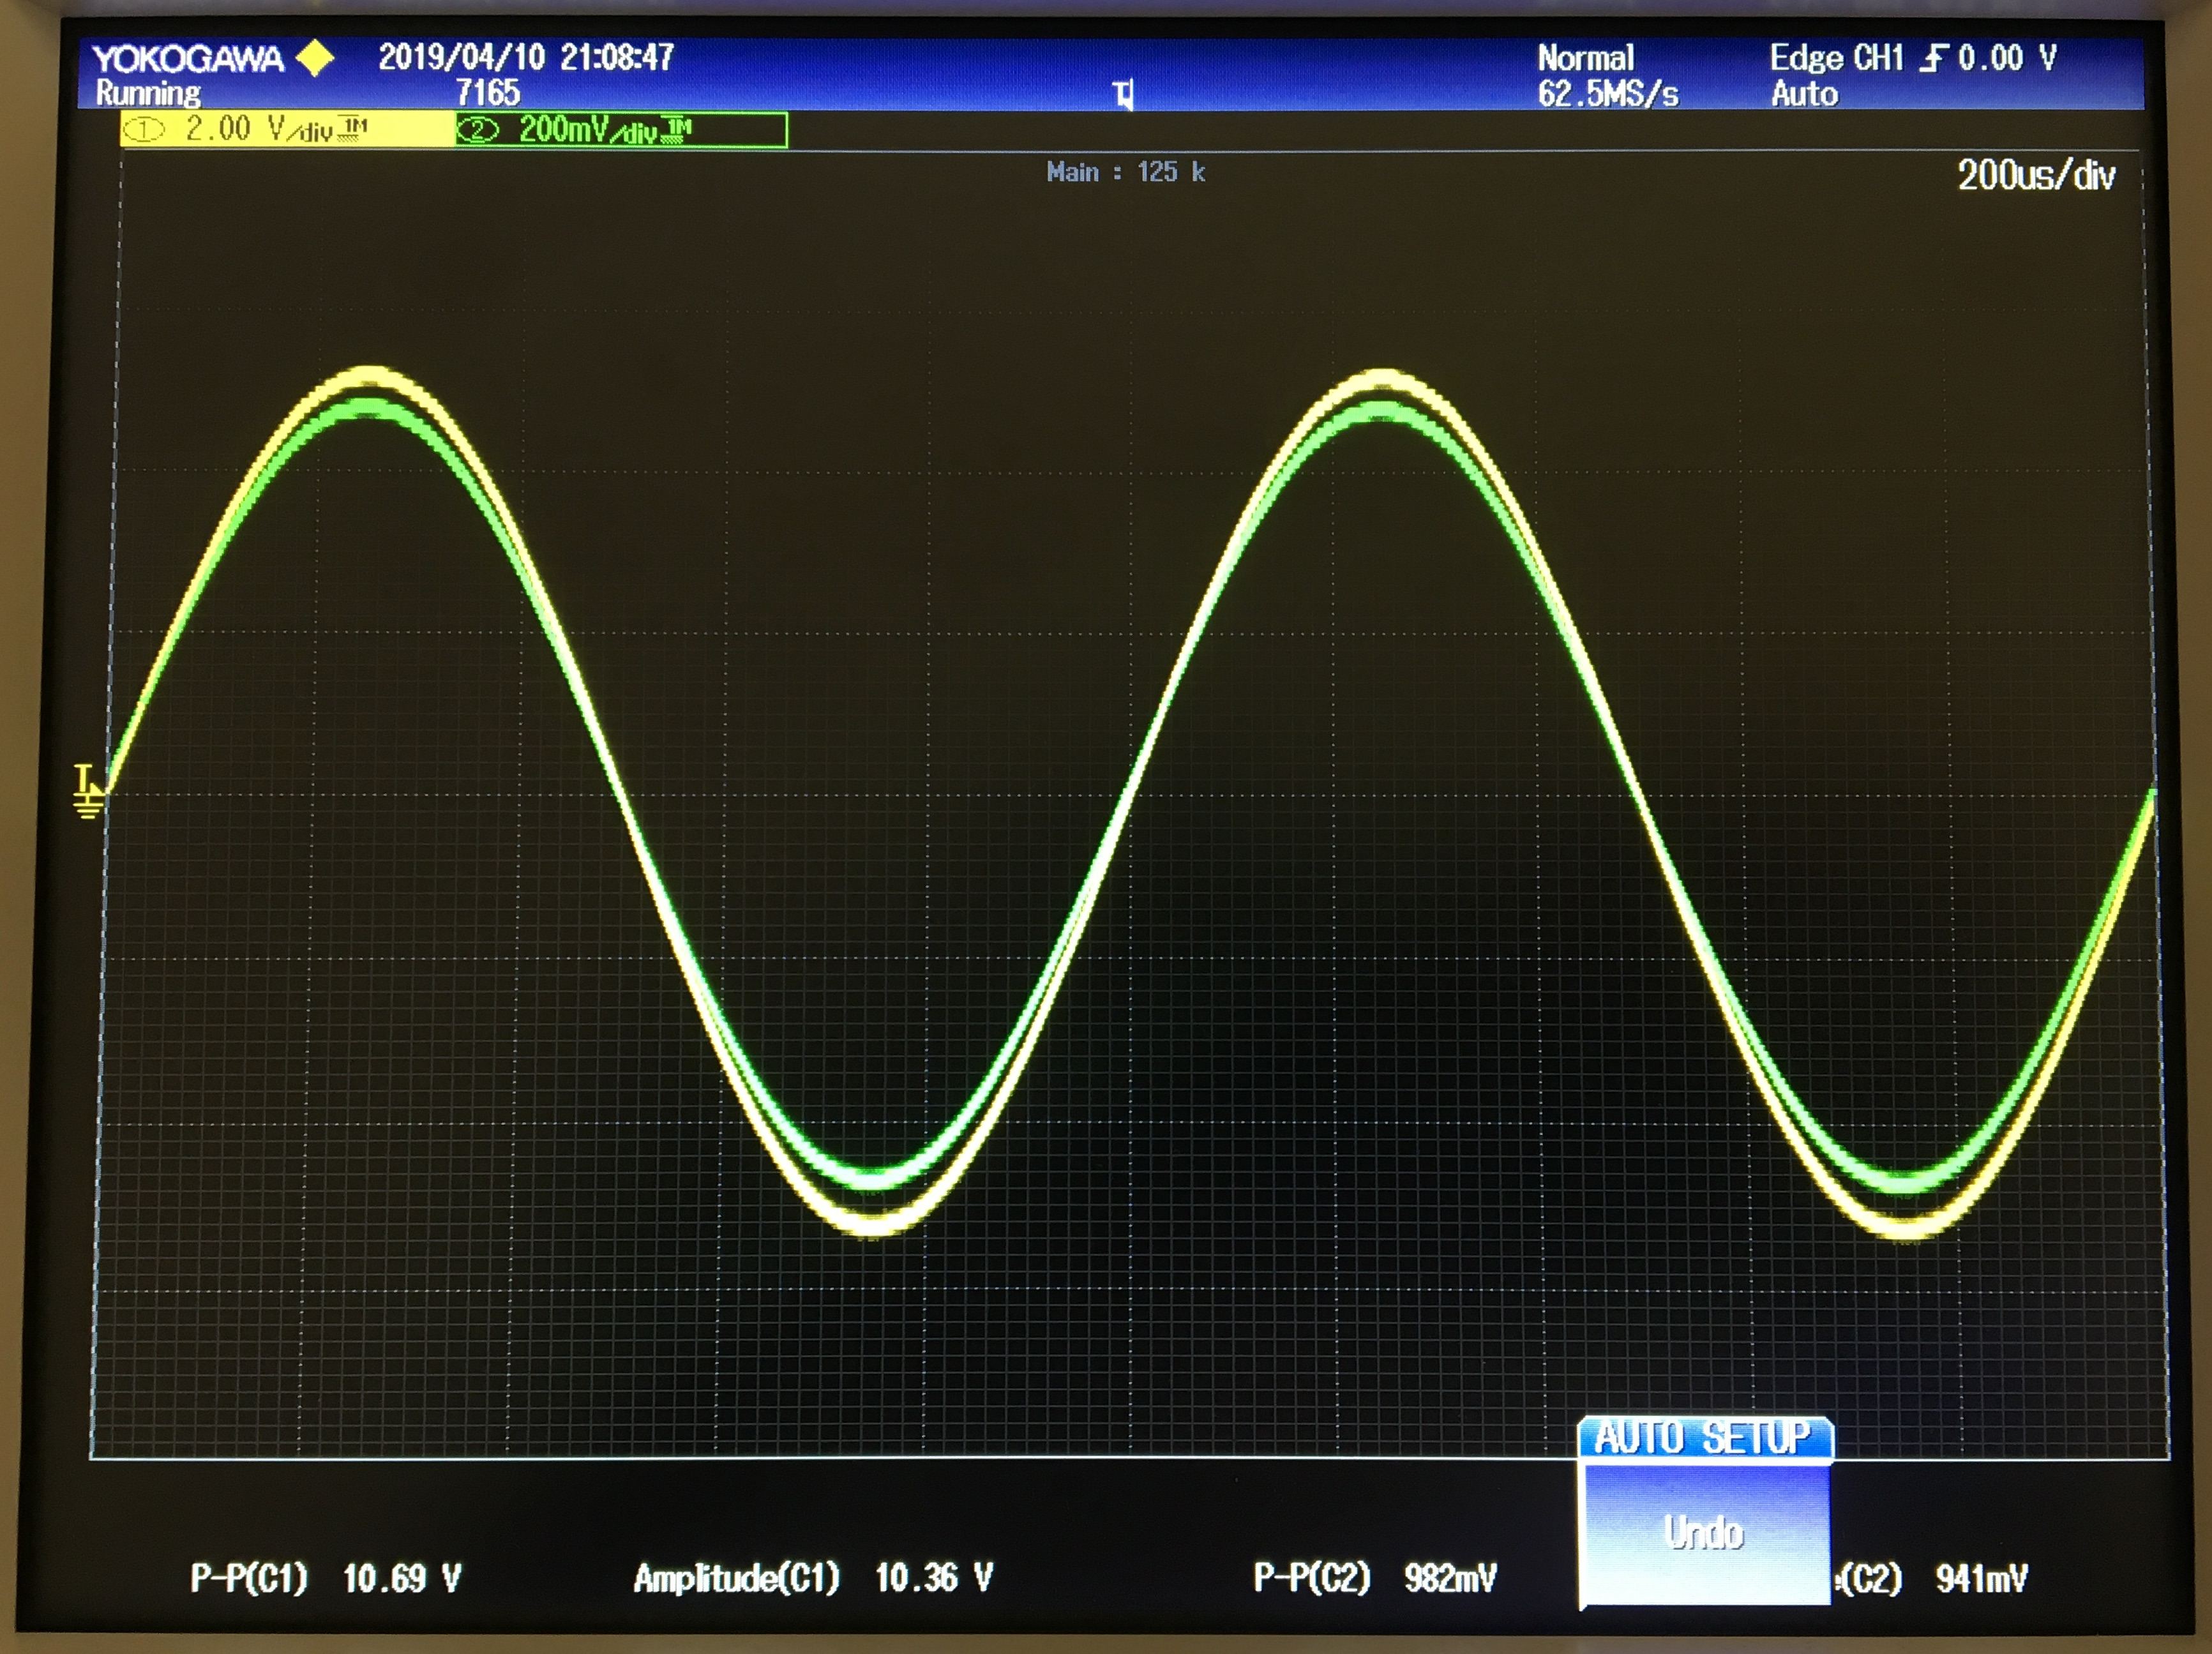
\includegraphics[width=\columnwidth]{images/lab7_non_inverting_osc.jpg}
    \captionof{figure}{Output of the non-inverting amplifier}
    \label{fig:non_inverting_osc}
    \medskip
\endgroup

\noindent Figure \ref{fig:summing_osc} shows the output for the summing amplifier. For this configuration, both input voltages were DC (at 5V and 3V), hence producing a flat output signal of \abs{8V}, as shown by the reading on the bottom left. The result verified previous calculations.

\begingroup
    \centering
    \medskip
    %width=\columnwidth
    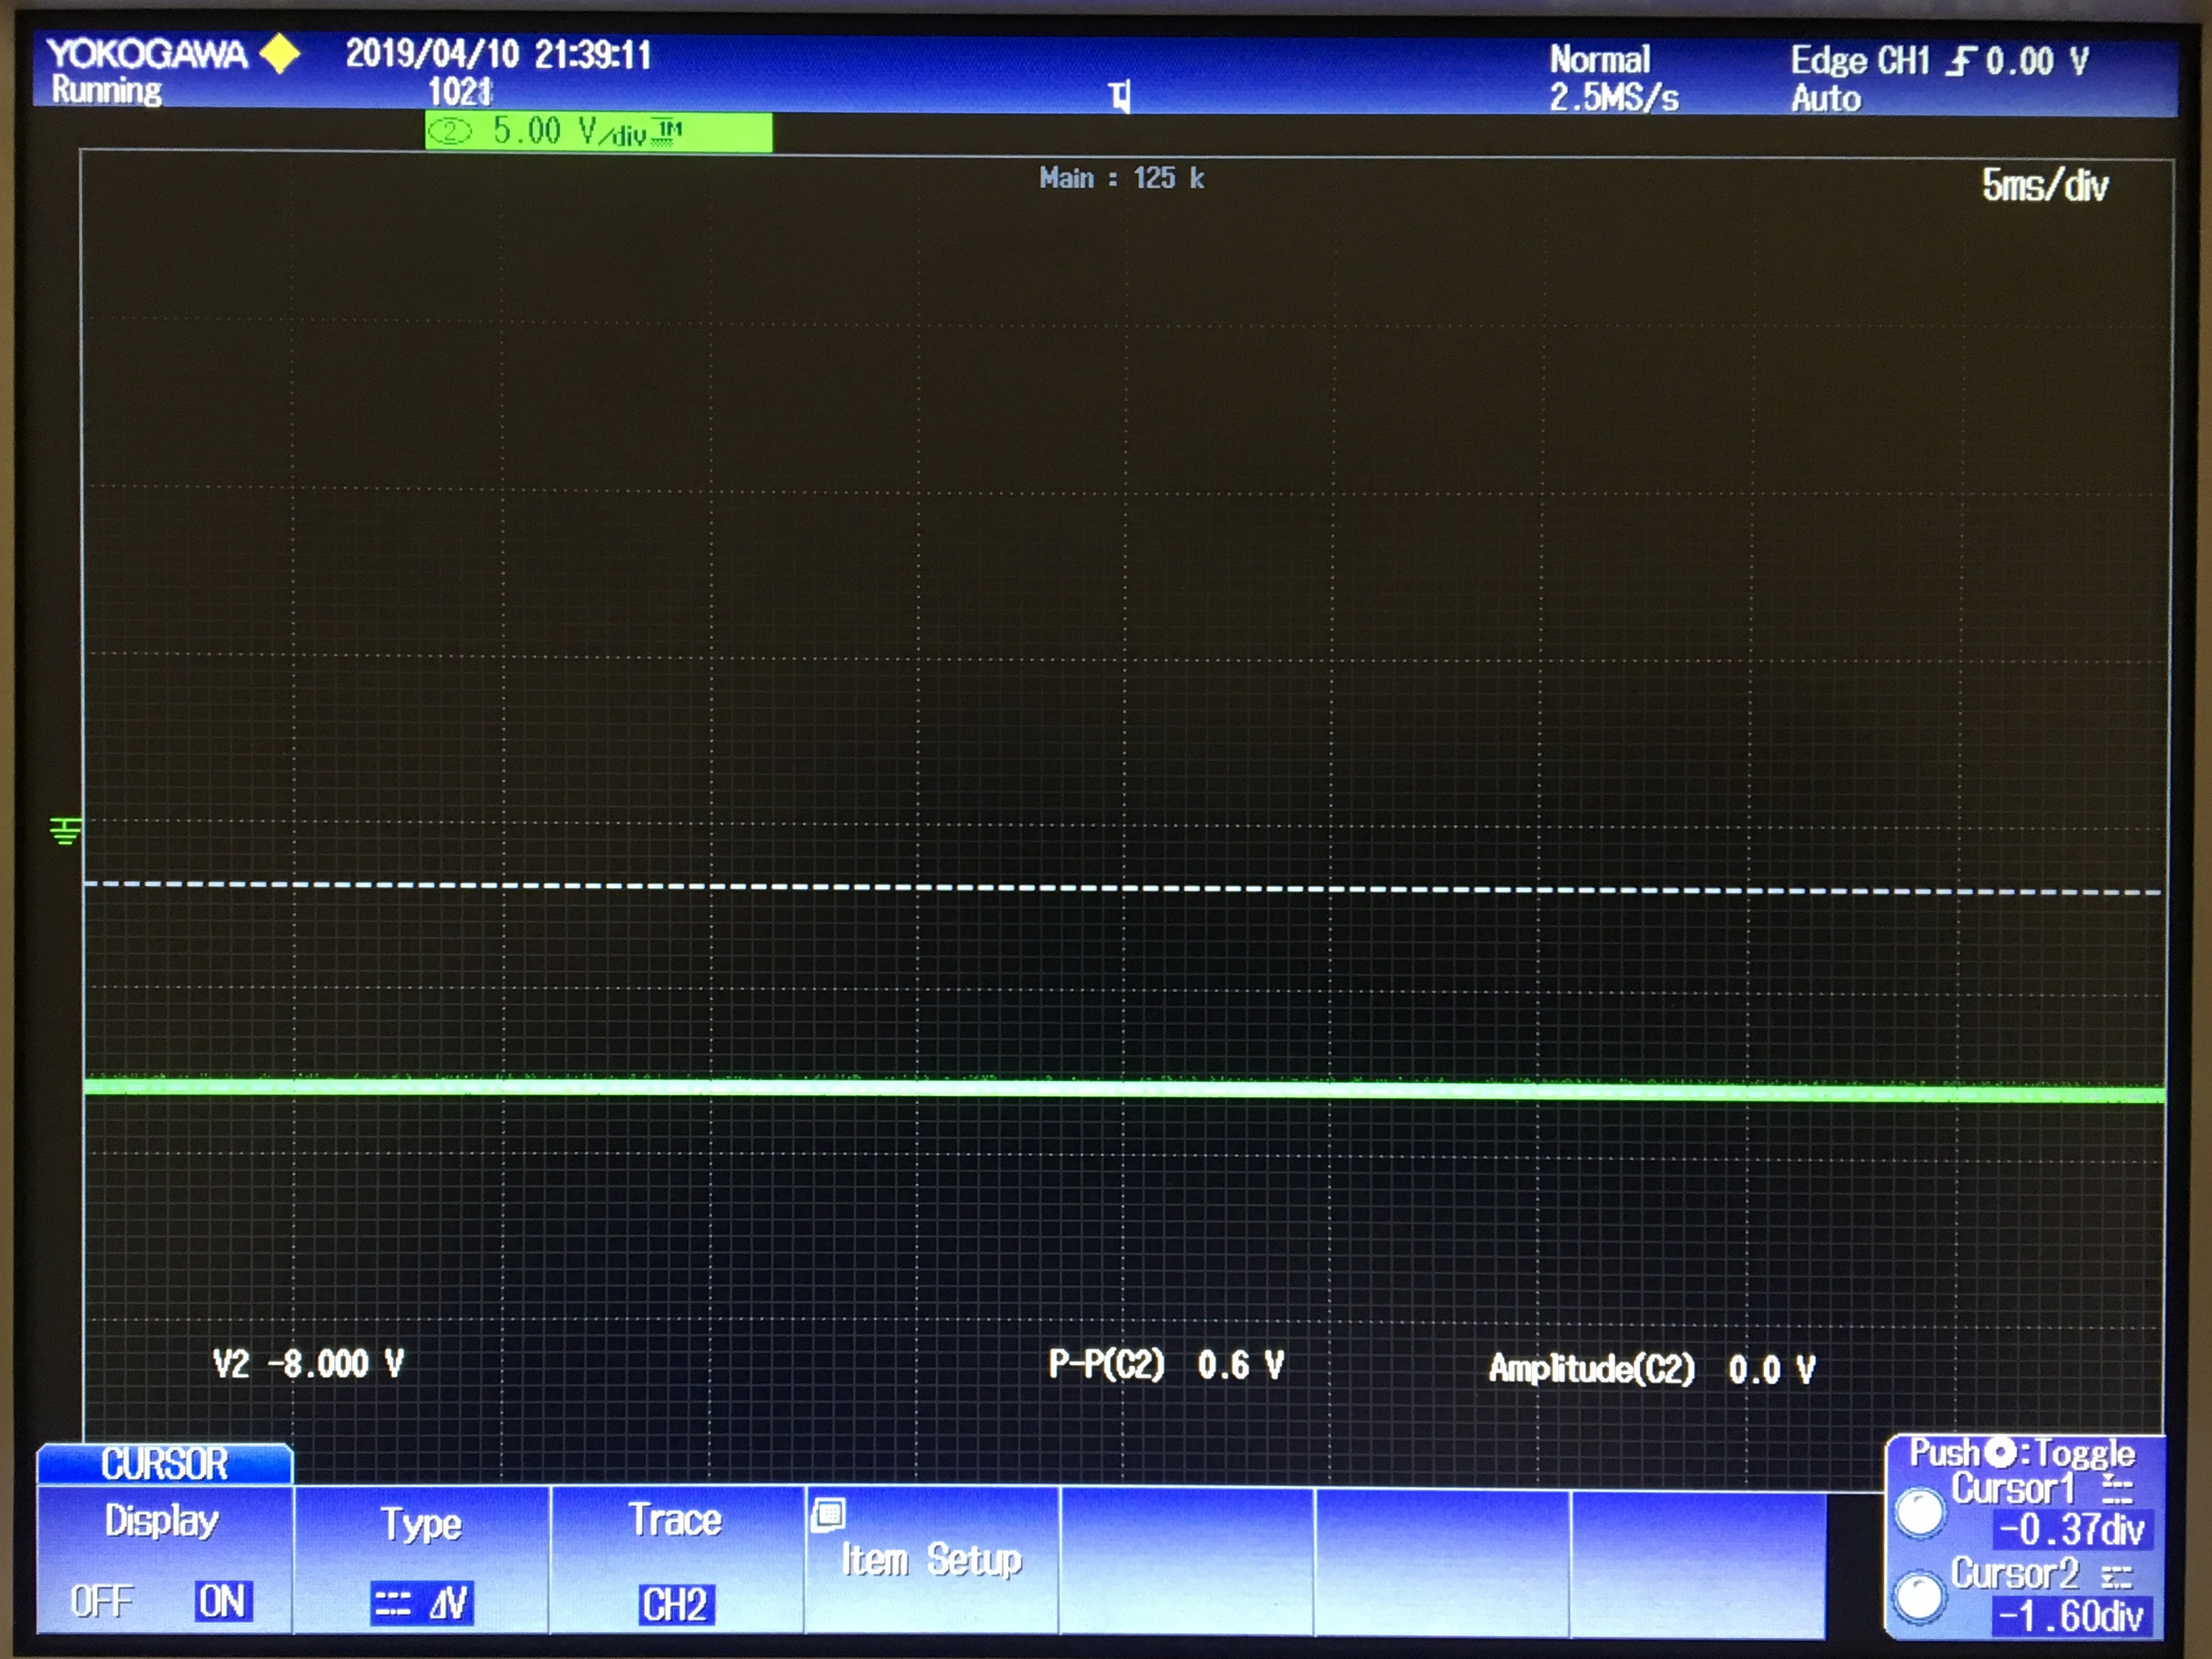
\includegraphics[width=\columnwidth]{images/lab7_summing_osc.jpg}
    \captionof{figure}{Output of the summing amplifier}
    \label{fig:summing_osc}
    \medskip
\endgroup

\noindent Finally, \ref{fig:cascading_osc} shows the output of the cascading amplifiers. Counting the divisions shows that the input signal had a voltage of approximately 1V, while the output signal had an output voltage of approximately 6V, confirming the predicted gain of 6.  

\begingroup
    \centering
    \medskip
    %width=\columnwidth
    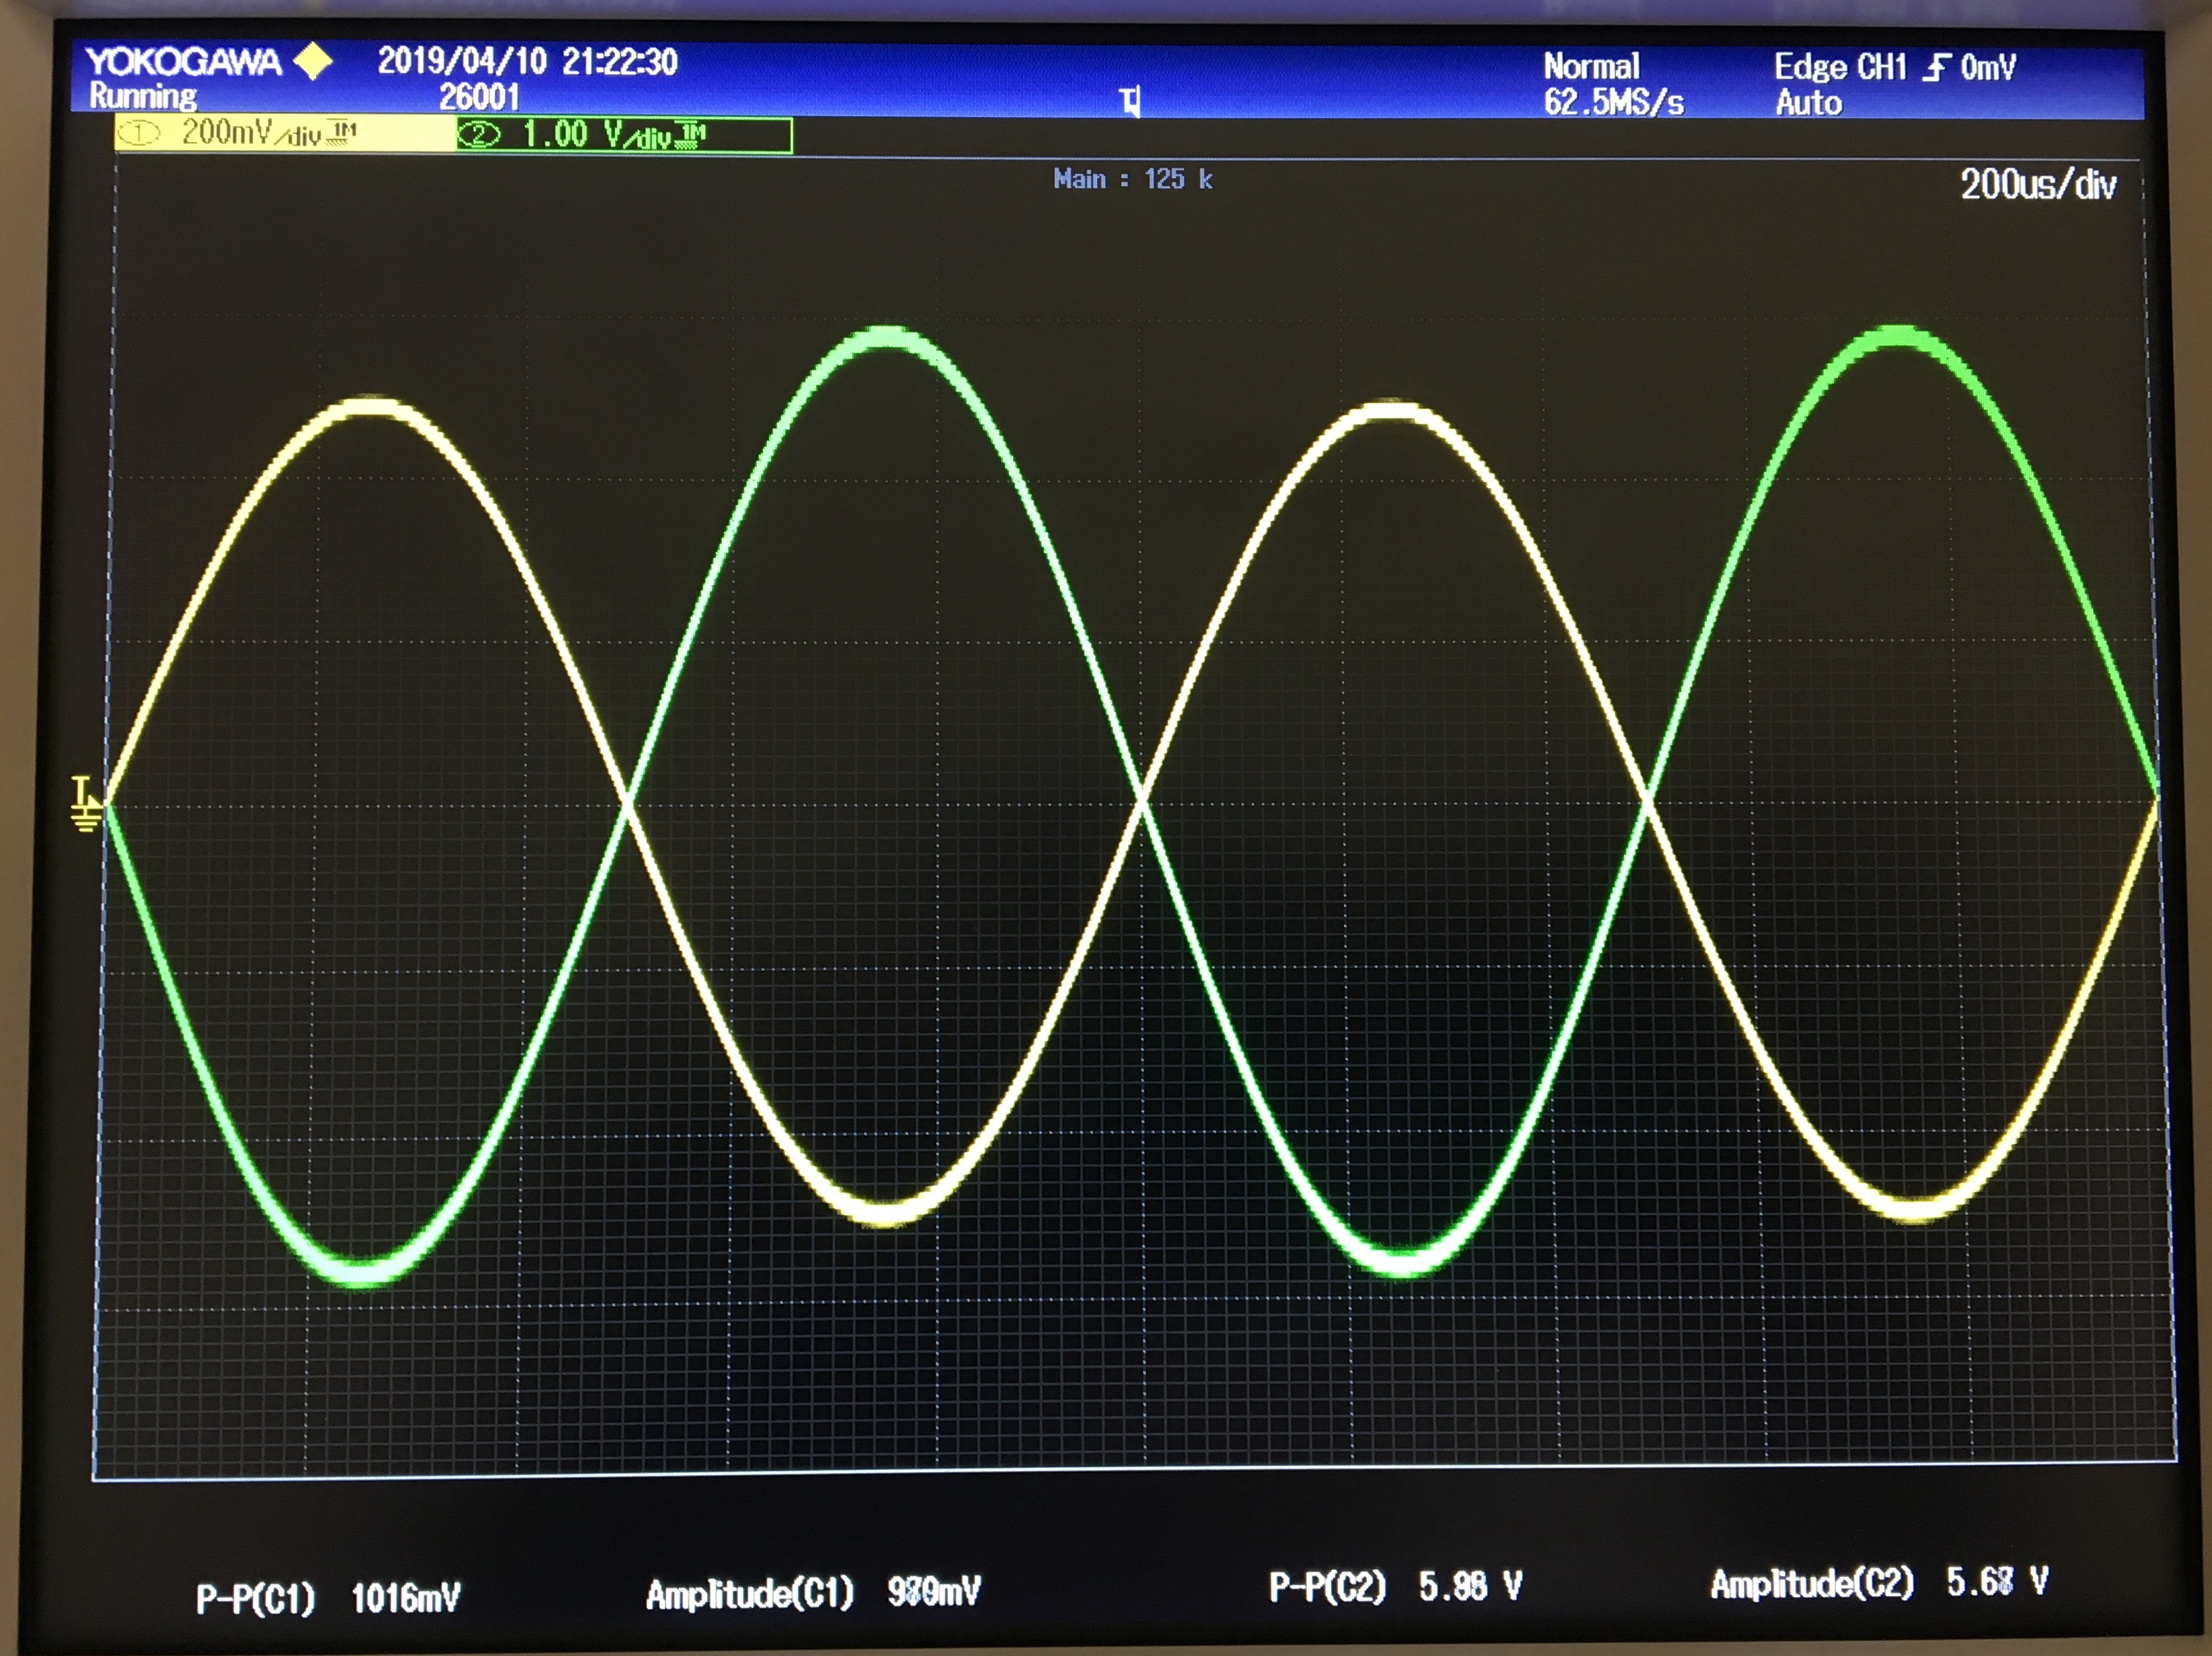
\includegraphics[width=\columnwidth]{images/lab7_cascading_osc.jpg}
    \captionof{figure}{Output of the cascading amplifier}
    \label{fig:cascading_osc}
    \medskip
\endgroup

\section{Conclusions}
% Understanding and applications
\noindent We learned two important things out of this experiment. Firstly, we accidentally used resistors with different values than suggested in the lab manual. As a result, we got more amplification than we needed as shown in Figure \ref{fig:fucked}. The yellow line represents the amplified result, and the green line represents the original signal. The generated signal was very close to a square wave. So, we learned that extreme amplification of the signal could be used to generate square waves and it can be useful in many applications with such requirement. For example, electric guitar amps clip signals near the edges to produce a distorted sound effect 

\begingroup
    \centering
    \medskip
    %width=\columnwidth
    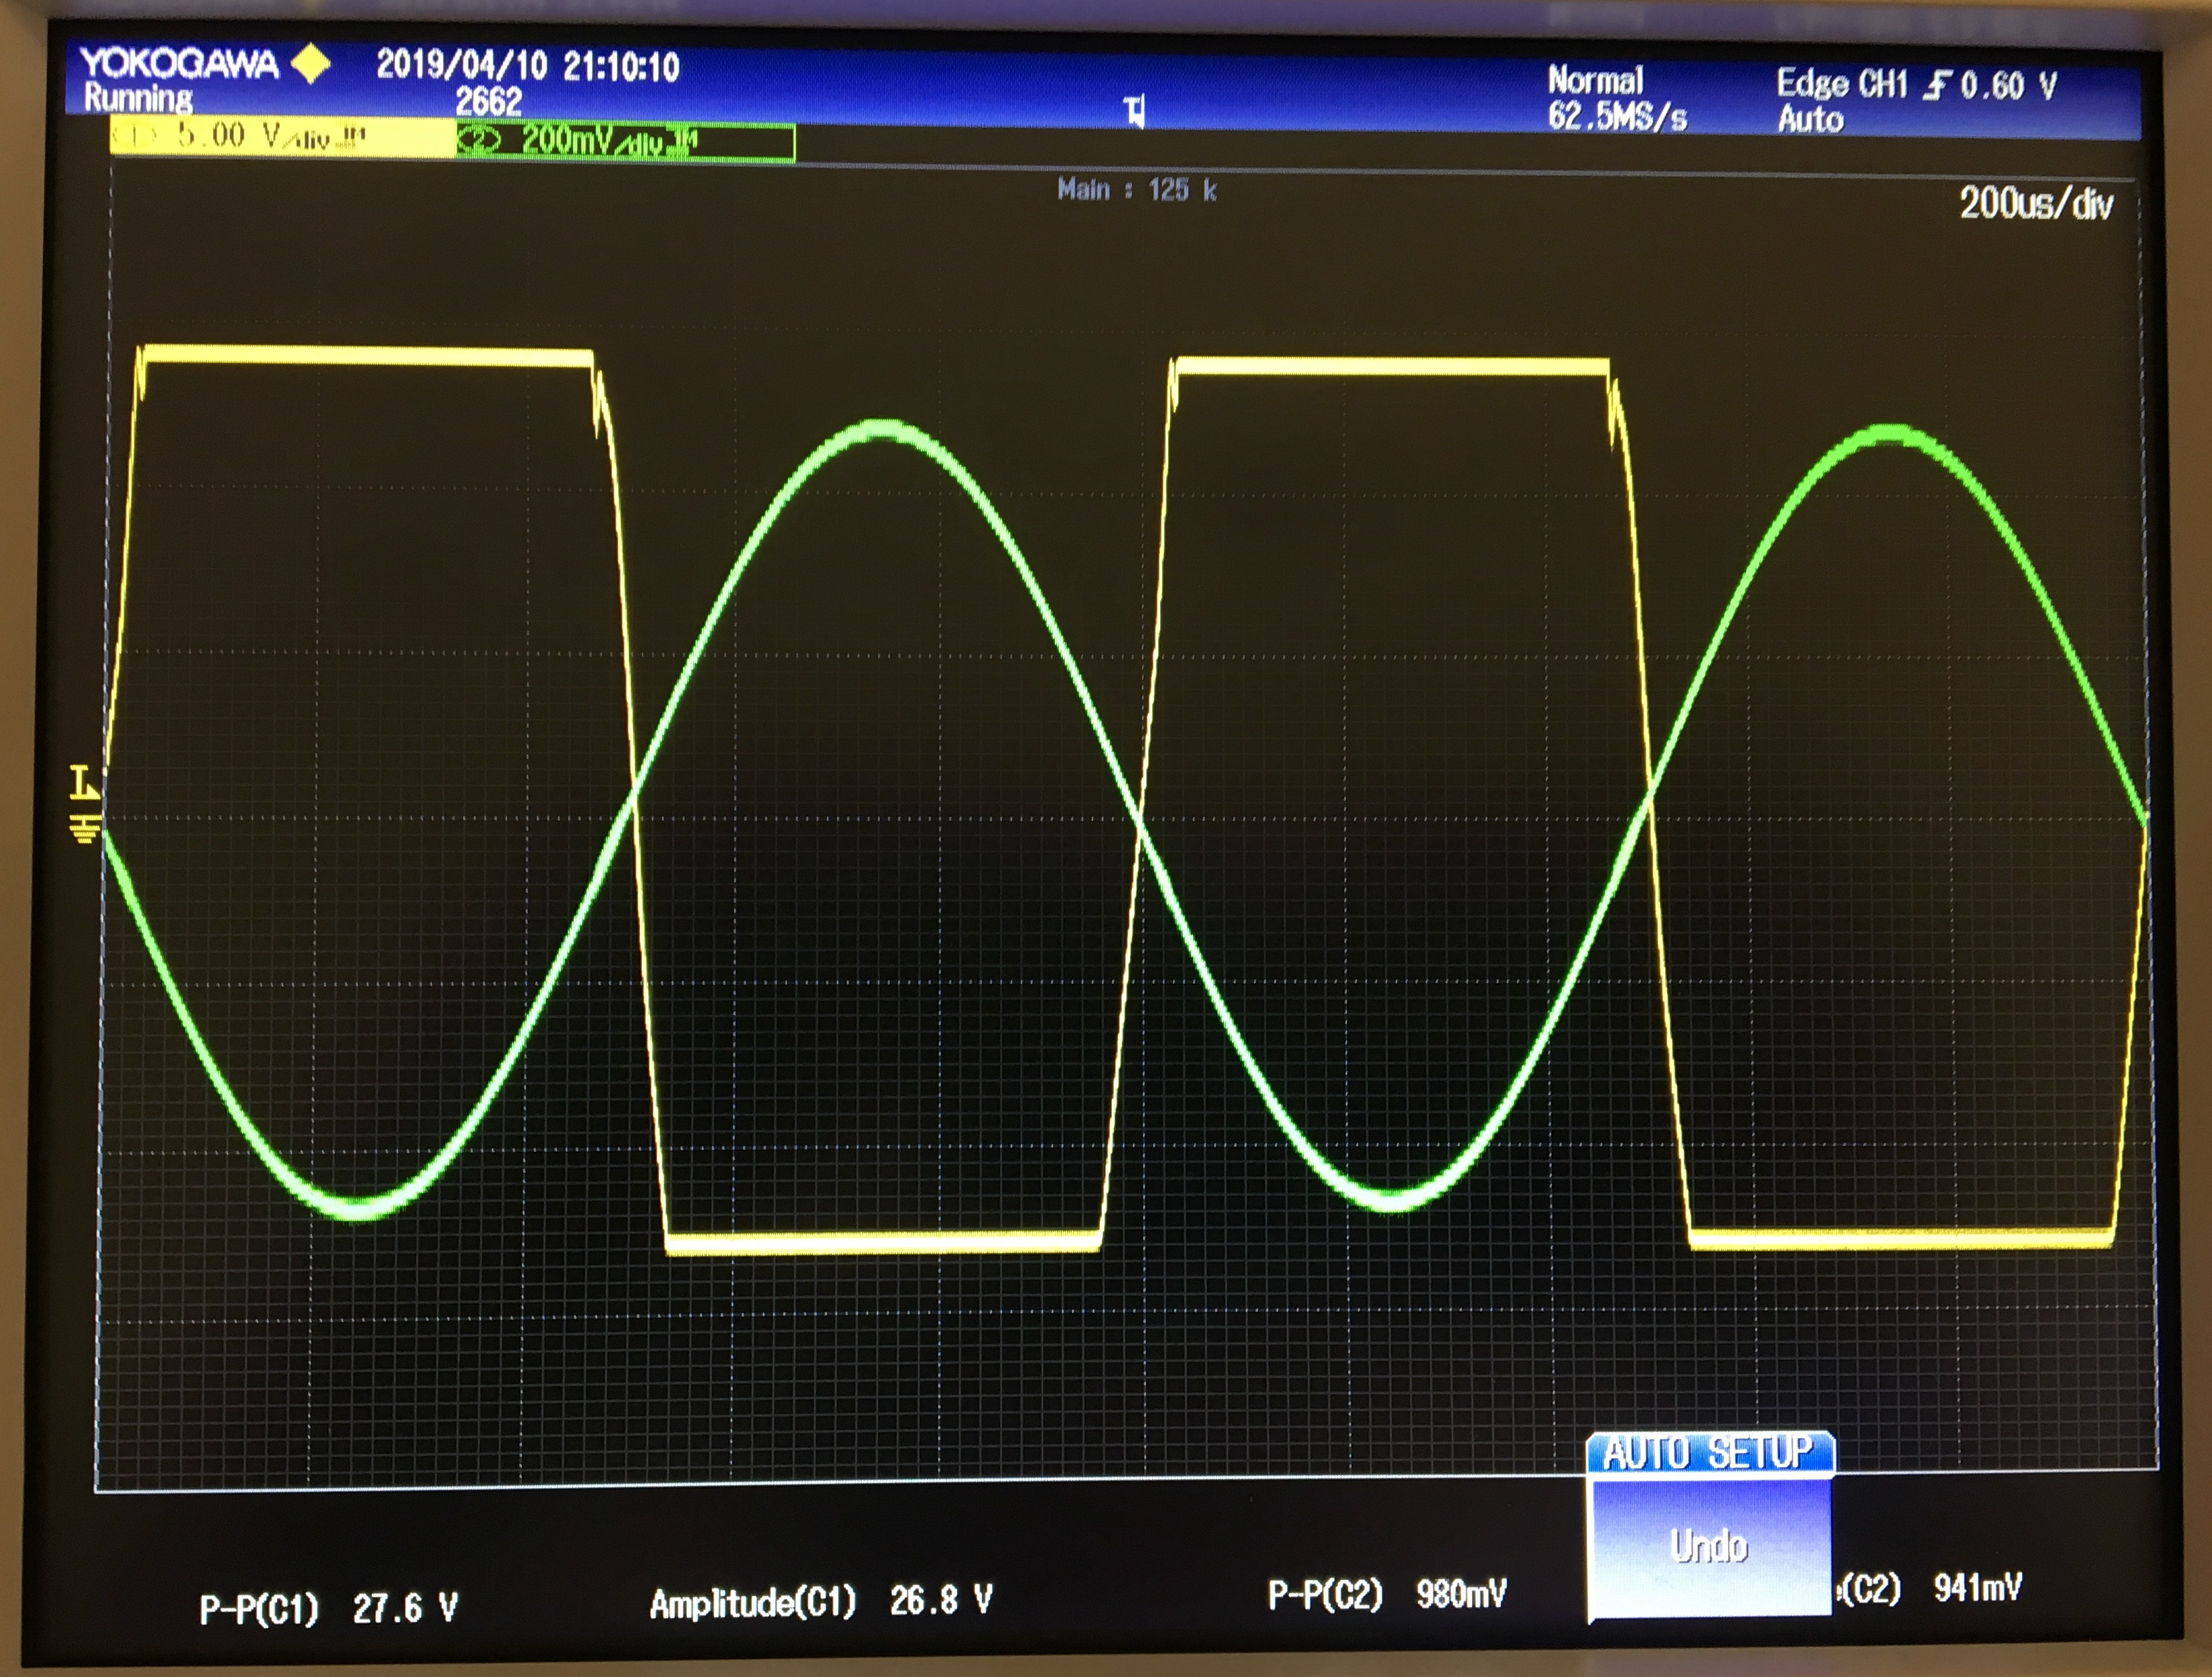
\includegraphics[width=\columnwidth]{images/lab7_fucked.jpg}
    \captionof{figure}{Output of the cascading amplifier}
    \label{fig:fucked}
    \medskip
\endgroup

\noindent Secondly, we forgot to connect the ground of the power supply used to power the opamp to the common ground. We assumed that having +15V and -15V was enough to run the circuit. However, we realized that we were not providing a reference value, namely ground, to the power supply and it was creating unwanted voltage values. We realized the importance of having a common ground. \\

\noindent Amplifiers are versatile devices with a variety of uses in industry, especially in audio applications. Inverting amplifiers have noise-cancelling applications, for example in headphones, where the input signal is inverted to cancel the unwanted noise. Non-inverting amplifiers are also widely used to increase the strength of signals received by a microphone, to relay to a speaker. Summing amplifiers are an ideal solution for audio mixers, as they are able to provide an output signal that is the sum of all input signals. Hence one can imagine several channels, such as voices and instruments, being fed into a summing amplifier and then fed into a non-inverting amplifier for signal strengthening. Cascading opamps are also common configurations for drastically improving gain; such configurations are also used to immediately increase the gain of the input signal so that it is not affected by other interference as it passed through other stages of signal processing. 

\printbibliography

\end{document}